% $Id: jfsample.tex,v 19:a118fd22993e 2013/05/24 04:57:55 stanton $
\documentclass[12pt,english,authoryear]{article}

% DEFAULT PACKAGE SETUP

\usepackage{setspace,graphicx,epstopdf,amsmath,amsfonts,amssymb,amsthm,versionPO}
\usepackage{marginnote,datetime,enumitem,subfigure,rotating,fancyvrb}
\usepackage{hyperref,float}
\usepackage[utf8x]{inputenc}
\usepackage{array}
\usepackage{makecell}
\usepackage{graphicx}
\usepackage{subfig}
\usepackage[english]{babel}
%\usepackage[style=apa,backend=biber,language=american]{biblatex}
%\DeclareLanguageMapping{american}{american-apa}

\usepackage[font=small,labelfont=bf]{caption}
\usepackage{apacite}
\usdate

% These next lines allow including or excluding different versions of text
% using versionPO.sty

\excludeversion{notes}		% Include notes?
\includeversion{links}          % Turn hyperlinks on?

% Turn off hyperlinking if links is excluded
\iflinks{}{\hypersetup{draft=true}}

% Notes options
\ifnotes{%
\usepackage[margin=1in,paperwidth=10in,right=2.5in]{geometry}%
\usepackage[textwidth=1.4in,shadow,colorinlistoftodos]{todonotes}%
}{%
\usepackage[margin=1in]{geometry}%
\usepackage[disable]{todonotes}%
}

% Allow todonotes inside footnotes without blowing up LaTeX
% Next command works but now notes can overlap. Instead, we'll define 
% a special footnote note command that performs this redefinition.
%\renewcommand{\marginpar}{\marginnote}%

% Save original definition of \marginpar
\let\oldmarginpar\marginpar

% Workaround for todonotes problem with natbib (To Do list title comes out wrong)
\makeatletter\let\chapter\@undefined\makeatother % Undefine \chapter for todonotes

% Define note commands
\newcommand{\smalltodo}[2][] {\todo[caption={#2}, size=\scriptsize, fancyline, #1] {\begin{spacing}{.5}#2\end{spacing}}}
\newcommand{\rhs}[2][]{\smalltodo[color=green!30,#1]{{\bf RS:} #2}}
\newcommand{\rhsnolist}[2][]{\smalltodo[nolist,color=green!30,#1]{{\bf RS:} #2}}
\newcommand{\rhsfn}[2][]{%  To be used in footnotes (and in floats)
\renewcommand{\marginpar}{\marginnote}%
\smalltodo[color=green!30,#1]{{\bf RS:} #2}%
\renewcommand{\marginpar}{\oldmarginpar}}
%\newcommand{\textnote}[1]{\ifnotes{{\noindent\color{red}#1}}{}}
\newcommand{\textnote}[1]{\ifnotes{{\colorbox{yellow}{{\color{red}#1}}}}{}}

% Command to start a new page, starting on odd-numbered page if twoside option 
% is selected above
\newcommand{\clearRHS}{\clearpage\thispagestyle{empty}\cleardoublepage\thispagestyle{plain}}

% Added by Daniel

\renewcommand\theadalign{bc}
\renewcommand\theadfont{\bfseries}
\renewcommand\theadgape{\Gape[4pt]}
\renewcommand\cellgape{\Gape[4pt]}
\renewcommand{\arraystretch}{1.5}
\usepackage{bm}
\interfootnotelinepenalty=10000
\usepackage{tocloft}
\addtolength{\cftsecnumwidth}{12pt}

% Number paragraphs and subparagraphs and include them in TOC
\setcounter{tocdepth}{2}

% JF-specific includes:

\usepackage{indentfirst} % Indent first sentence of a new section.
\usepackage{endnotes}    % Use endnotes instead of footnotes
\usepackage{jf}          % JF-specific formatting of sections, etc.
\usepackage[labelfont=bf,labelsep=period]{caption}   % Format figure captions
\captionsetup[table]{labelsep=none}

% Define theorem-like commands and a few random function names.
\newtheorem{condition}{CONDITION}
\newtheorem{corollary}{COROLLARY}
\newtheorem{proposition}{PROPOSITION}
\newtheorem{obs}{OBSERVATION}
\newcommand{\argmax}{\mathop{\rm arg\,max}}
\newcommand{\sign}{\mathop{\rm sign}}
\newcommand{\defeq}{\stackrel{\rm def}{=}}

\begin{document}

\setlist{noitemsep}  % Reduce space between list items (itemize, enumerate, etc.)
\onehalfspacing      % Use 1.5 spacing
% Use endnotes instead of footnotes - redefine \footnote command
\renewcommand{\footnote}{\endnote}  % Endnotes instead of footnotes

% Change the table numbering to regular numbers

\renewcommand{\thetable}{\arabic{table}}

\author{Daniël Steman (2633103)\thanks{\rm MS Finance: Duisenberg Honours Programme in Finance \& Technology, School of Business and Economics, VU University Amsterdam.}\\[1cm]{\small Supervisor: dr. Jan Wrampelmeyer}}

\title{\Large \bf A High-Frequency Cointegration-Based Pair Trading System for the Cryptocurrency Market}

% Create title page with no page number

\maketitle
\thispagestyle{empty}

\medskip

\begin{center}

\includegraphics[width=12cm]{VU-University-Amsterdam-logo.png}
\end{center}

\medskip

%\noindent JEL classification: XXX, YYY.

\clearpage

\centerline{\bf ABSTRACT}

\begin{doublespace}  % Double-space the abstract and don't indent it
  \noindent In this paper, a high frequency pair trading system is proposed and its ability to yield a positive risk-adjusted return is tested with a sample of minute-binned exchange rates from 01-11-2019 until 29-03-2020. In the first month of the sample, long-run relationships are estimated by means of the two-stage Engle-Granger procedure and Johansen procedure, accounting for the multiple comparison problem \cite{Engle_1987, Johansen_1988, Seong_2009}. In the four months thereafter, five regimes of trading systems with varying thresholds are tested. The most successful trading system yields a cumulative return of 16.88\%, a Sharpe ratio of 1.68 and a return over maximum drawdown ratio of 2.12. The proposed strategy was especially profitable in February and March, when the cryptocurrency market performed poorly. The same is observed with regard to the S\&P500, showing market neutrality to some extent and offering diversification benefits to investors. Moreover, it is found that a statistical stop-loss mechanism can limit the magnitude of losses. The results put doubt on weak-form market efficiency of the cryptocurrency market. 
  
\end{doublespace}

\clearpage

\tableofcontents

\clearpage

% ############################################################################################################
\section{Introduction} \label{sec:Introduction}

The expanding universe of cryptocurrencies draws the attention of not only economists, governments and academics, but also high frequency traders who continuously seek to exploit the next undiscovered edge in the market. A popular strategy that relies solely on historical prices and speculates on short-term movements goes by the name of “pair trading". Two assets that have been comoving in the past are expected to comove in the future, so the spread between the two assets is expected to be stationary. Deviations from the spread open trading opportunities: short the asset that outperforms and long the asset that underperforms. When the spread converges, the positions are reversed and a profit is locked in. 

The efficient market hypothesis states that prices in the market reflect all information and the weak form of this hypothesis states that prices reflect all data of past prices. If the cryptocurrency market is weakly efficient, a pair trading strategy should not be able to generate a positive risk-adjusted return. However, the cryptocurrency market is still in its infancy, lacks regulation and is dominated by sentiment. Therefore, it is expected that it is possible to achieve a positive risk-adjusted return with the trading system that is proposed in this paper. The performance of the strategy is tested with a high frequency sample of minute-binned exchange rates from November, 2019 until March, 2020. 

In the first stage of the paper, long term relationships between cryptocurrency exchange rates are estimated using two approaches to test cointegration, namely the two-stage Engle-Granger \citeyear{Engle_1987} procedure and the Johansen \citeyear{Johansen_1988} procedure. Given previously observed signs of comovement and interdependence of cryptocurrencies, it was expected that there are statistically significant cointegrated exchange rates that can be used in the proceeding steps. However, due to the volatility observed in the past, it is also expected that cointegrating relationships may not hold over time, something that affects the performance of the strategy. Despite the strict pair selection process, 8 out of 55 pairs of exchange rates are determined to be significantly cointegrated in the month preceding the backtesting period.

In the second stage, five trading systems with varying thresholds are backtested in a period of four months. The dynamics of each system are analysed in terms of trading frequency, profit-and-loss, return and risk. 

Stop-loss orders are usually implemented to limit the loss in a position. Previous literature suggests that the integration of a stop loss order in a pair trading strategy in the cryptocurrency market contaminates profits, because it does not fully capture the mean-reverting characteristic of the spread. As an extension, the benefit of an alternative stop-loss mechanism based on a rolling window unit root test is explored. To the best of my knowledge, this variation of a stop-loss order has not been addressed by literature to date.  
The results show that the trading system with $\pm$ one standard deviation from the mean spread is the most successful in terms of risk-adjusted return. Cointegrating relationships of pairs changed over time, as the market got exposed to shocks. As a consequence, the portfolio suffered losses during two months, but made up for it in the months when the market stabilized. With a four-month return of 16.88\% and an annualized Sharpe ratio of 1.68, it outperformed the equity market. The portfolio returns are not correlated to either the cryptocurrency market or the equity market, offering diversification benefits to investors. The pair trading strategy solely relies on past price data and yielded excess returns, implying that weak-form market efficiency of the cryptocurrency market is questionable. 

The paper is structured in a number of sections, starting off with background information of cryptocurrencies in \hyperref[sec:Background]{section 2}, followed by a presentation and discussion of relevant literature in \hyperref[sec:Literature]{section 3}. The data set is explored and discussed in \hyperref[sec:Data]{section 4}. The methods that are applied to test cointegration, the trading rules and assessment are discussed in \hyperref[Method]{section 5}. The results of are presented and discussed in \hyperref[sec:Results]{section 6}, followed by an extension to the research in \hyperref[sec:Extension]{section 7}. The paper ends with a conclusion in \hyperref[sec:Conclusion]{section 8}. 

% ############################################################################################################
\section{Background} \label{sec:Background}

Originally introduced in 2008 under the pseudonym Satoshi Nakamoto, Bitcoin is a cryptocurrency derived from mathematical cryptography and is unique due to its decentralised nature. Bitcoins are generated by individuals who solve complex computational problems and contribute to the blockchain \cite{Nakamoto2008}. The universe of cryptocurrencies expanded in 2017 with a large number of initial coin offerings (ICO). An ICO is similar to an initial public offering (IPO), but is for cryptocurrencies and \textit{tokens} and serve as a channel of crowdfunding for start-ups. The digital assets that arise from these ICOs are called \textit{altcoins} and are based on new versions of the blockchain. 

Alternatively, when there is no consensus on the existing blockchain, a hard fork may give birth to a new altcoin, such as the popular Litecoin that was founded three years after the origin of Bitcoin. Blockchain validation software can be upgraded with new validation rules. Usually, all nodes in the network will adhere to the new validation rules by upgrading their blockchain validation software. However, there can be nodes that will continue to validate the blockchain using the old validation rules. Blocks produced according to the new validation rule are classified as invalid. This gives rise to two blockchains: the original and a variation of the original (e.g. Bitcoin and Bitcoin Cash)

Once initiated, Bitcoins and altcoins are traded on the secondary market. At the time of writing, Bitcoin has a market capitalisation of 179.8 billion U.S. dollars and the aggregate of all cryptocurrencies amounts to a market capitalisation of 277.5 billion U.S. dollars \cite{CMC}. Trade of cryptocurrencies is facilitated by more than 300 exchanges. Binance is the exchange of choice in this paper because it is the largest exchange in terms of traded volume, so illiquidity will not be a constraint. 

The cryptocurrency market shows resemblance with the FX market in that they are both decentralised market places where currencies can be traded at any time of the day. The FX market has existed since the invention of national currency, which means that the market is matured. With approximately 95\% of FX traders being institutions, the market is highly competitive and efficient. The relatively new cryptocurrency market is predominantly home to retail investors, is more volatile and has lower transaction fees. These are favorable characteristics for a high frequency pair trading strategy that opens many positions and derives its profitability from short-term deviations.

Because converting fiat currency to cryptocurrency is not possible for all currencies and is often subject to high transaction fees, all cryptocurrencies will be quoted in USDT (Tether), which is the most widely used stable coin on Binance and many other exchanges (www.tether.to). A stable coin is a cryptocurrency with minimal volatility and is usually pegged against a fiat currency or a basket of stable assets, in the case of Tether that is the U.S. dollar.

% ############################################################################################################
\section{Literature} \label{sec:Literature}

Quantitative trading has become a buzzword in the field of modern finance. Exponential growing computing power combined with ever volatile markets (at the time of writing) open up opportunities that are closed by high frequency traders within milliseconds. A widely exploited strategy is pair trading, which is a mathematical analysis based trading strategy that trades two securities with an economic or statistical relationship. In practice, one would sell the outperforming security and one would buy the underperforming security relative to the constant spread. When the positions are reversed, a profit can be made \cite{Gatev2006, Vidamurthy_2004}. Given the nature of this strategy, an investor can profit from uptrends and downtrends, hence it is a market neutral strategy \cite{Elliot_2007}. While the investor base of the cryptocurrency market is growing, there has been little research on the potential of a pair trading strategy in the relatively new market.

Successful implementation of a pair trading strategy relies on comovement that is caused by a statistical or economical relationship between two assets. Some claim that there are no economic relationships in the cryptocurrency market and that prices are merely inflated by speculative bubbles, hence the high volatility observed in cryptocurrency markets \cite{Cheah_2015}. The lack of economic relationships among cryptocurrencies due to the non-existence of fundamental value poses a challenge for finding pairs eligible for trading. In the equity market, comovement is decoupled from fundamental value and is attributed to market frictions and noise trader sentiment \cite{Barbaris_2005}. Without fundamental value, one could argue that market friction and noise trader sentiment are the primary sources of comovement in the cryptocurrency market. This also supports findings that the cryptocurrency market is inefficient \cite{Urquhart_2016}. If comovement in the cryptocurrency market relies on market friction and noise trader sentiment, it is expected that cointegrating relationships are not robust, as they depend on forces that are difficult to measure. This calls for precaution in the second stage of the research. 

As opposed to equity markets, cryptocurrency markets are not regulated. Without a regulator that mitigates information asymmetry and adverse selection, noise traders are free to take on excessive risk, aggravating market inefficiency \cite{Delong_1990}. This puts more pressure on the robustness of the cointegrating relationships of pairs. Other research concludes that price, volume and volatility in cryptocurrency markets do revert in the short run, in case of a ‘pump-and-dump’ scenario \cite{Li_2019}. Pumps are likely to be driven by overconfident investors who belief they have the ability to time the market better than others. The valuation of overconfident traders exceeds the fundamental value because they belief the asset can be sold in the future for a higher price. If the impact of overconfident traders is sufficient, a speculative bubble can exist \cite{Scheikman_2003}. This is what happened in 2018, when Bitcoin lost one-third of its value in one week after a year of rapid price increases. 

Bitcoin is a de facto gold standard within the universe of cryptocurrencies, but there are many variations. At the time of writing, more than 5,000 altcoins are listed on websites such as coinmarketcap.com and messari.io. High correlations between cryptocurrencies have been observed by Aslandis, Bariviera and Martinez-Ibanez \citeyear{Aslanidis_2019} and Burnie \citeyear{Burnie_2018}. Additionally, Burnie finds that cryptocurrencies that are a fork of another cryptocurrency’s codebase show robust, strong, positive associations. Similarities in the blueprints of cryptocurrencies form an alternative explanation for the comovement that is observed in historical price data and may assist in identifying cointegrated pairs. Moreover, a hard fork can explain dissolving cointegrating relationships. 

Empirical findings show that there are large return and volatility spillovers due to the interconnectedness of the cryptocurrency market, with Bitcoin and Litecoin at its core and the second largest cryptocurrency, Ethereum, as a recipient of the spillovers \cite{Ji_2019}. In addition to interconnectedness among cryptocurrencies, it is also found that they are isolated from other financial assets, thus offering diversification opportunities \cite{Corbet_2018}. The cryptocurrency market and financial market are not completely isolated, because investors will move away from risky cryptocurrencies towards safer financial assets in crisis periods \cite{Matkovskyy_2019}. The interconnectedness that is found in the cryptocurrency market raises the chance of finding cointegrated pairs and supports the discovery of the potential of a pair trading strategy.

Krauss \citeyear{Krauss_2017} has reviewed the literature framework of relative-value arbitrage strategies that trade two or more securities, i.e. pair trading. Pair trading strategies are split in five streams. The distance approach evaluates the distance between prices over time to identify comoving securities. The cointegration approach uses a cointegration test to identify a long run equilibrium relationship, which is usually more reliable than the relationship that is identified with the distance approach. The time-series approach focuses on generating optimised trading signals through time-series analyses. The stochastic control approach is similar to the time-series approach and tries to find optimal portfolio holdings of the securities that compose a pair. There are many more approaches that include machine learning, principal component analysis and more. For this research I will focus on a cointegration approach which has shown to consistently deliver long-run equilibrium relationship estimates \cite{Inder_1993}.

Leung and Nguyen \citeyear{Leung_2018} implemented a cointegration-based pair trading strategy using daily price data of four liquid cryptocurrencies and found that the Engle-Granger procedure is preferred over the Johansen procedure, because it mean-reverts faster, making trades more frequently which translates into improved risk-adjusted returns. They also found that a trading system without a stop-loss or trailing backstop yields the highest returns because it fully captures the mean-reversion dynamic, while the use of a stop-loss or trailing backstop contaminates the profit-and-loss (PnL). Miao \citeyear{Miao_2014} yields the highest returns with an open-trade condition at two standard deviation away from the mean and a stop-loss that closes positions when the spread crosses 4 standard deviations.

The proposed high frequency pair trading strategy solely bases its predictions on historical data, putting doubt on weak form market efficiency. In matured, highly competitive and efficient equity markets and FX markets, it is not expect that the proposed strategy has the ability to generate a positive risk-adjusted return. On the contrary, the cryptocurrency market is found the be inefficient, primarily explained by its infancy, and most digital assets are highly correlated, which raises the chance of finding cointegrated pairs. These properties make the cryptocurrency market a promising environment and it is expected that the proposed strategy has the potential to generate a positive risk-adjusted return. 

% ############################################################################################################
\section{Data} \label{sec:Data}

Data has been provided by Kaiko, a Paris based cryptocurrency data provider, for academic purposes. The data set contains the open, high, low, close and volume (OHLCV) per minute from 01-11-2019 00:00 until 29-03-2020 23:59 for all cryptocurrencies traded on the Binance exchange. To avoid survivorship bias when picking exchange rates for trading, I picked the top 20 cryptocurrency exchange rates based on volume on the first day of the data set, which is 01-11-2019, from Coinmarketcap. Fourteen of these exchange rates are traded on the Binance exchange, eleven of which have less than 20\% missing values. The missing values are mostly clustered in less liquid exchange rates and are excluded from the data set to mitigate the risk of misinterpreting trading signals due to hidden price movements. For the remaining exchange rates, missing values are filled with the previously known value.

% Figure 1
\begin{center}
\begin{minipage}{\textwidth}
\captionof{figure}{Correlation matrix}
\caption*{\footnotesize The correlation heat map shows the associations between the cryptocurrency exchange rates with respect to USDT in the full data set, ranging from 01-11-2019 00:00 until 29-03-2020 00:00. Note that the color map is scaled to the smallest and largest correlation coefficient to visualise the relative differences.}
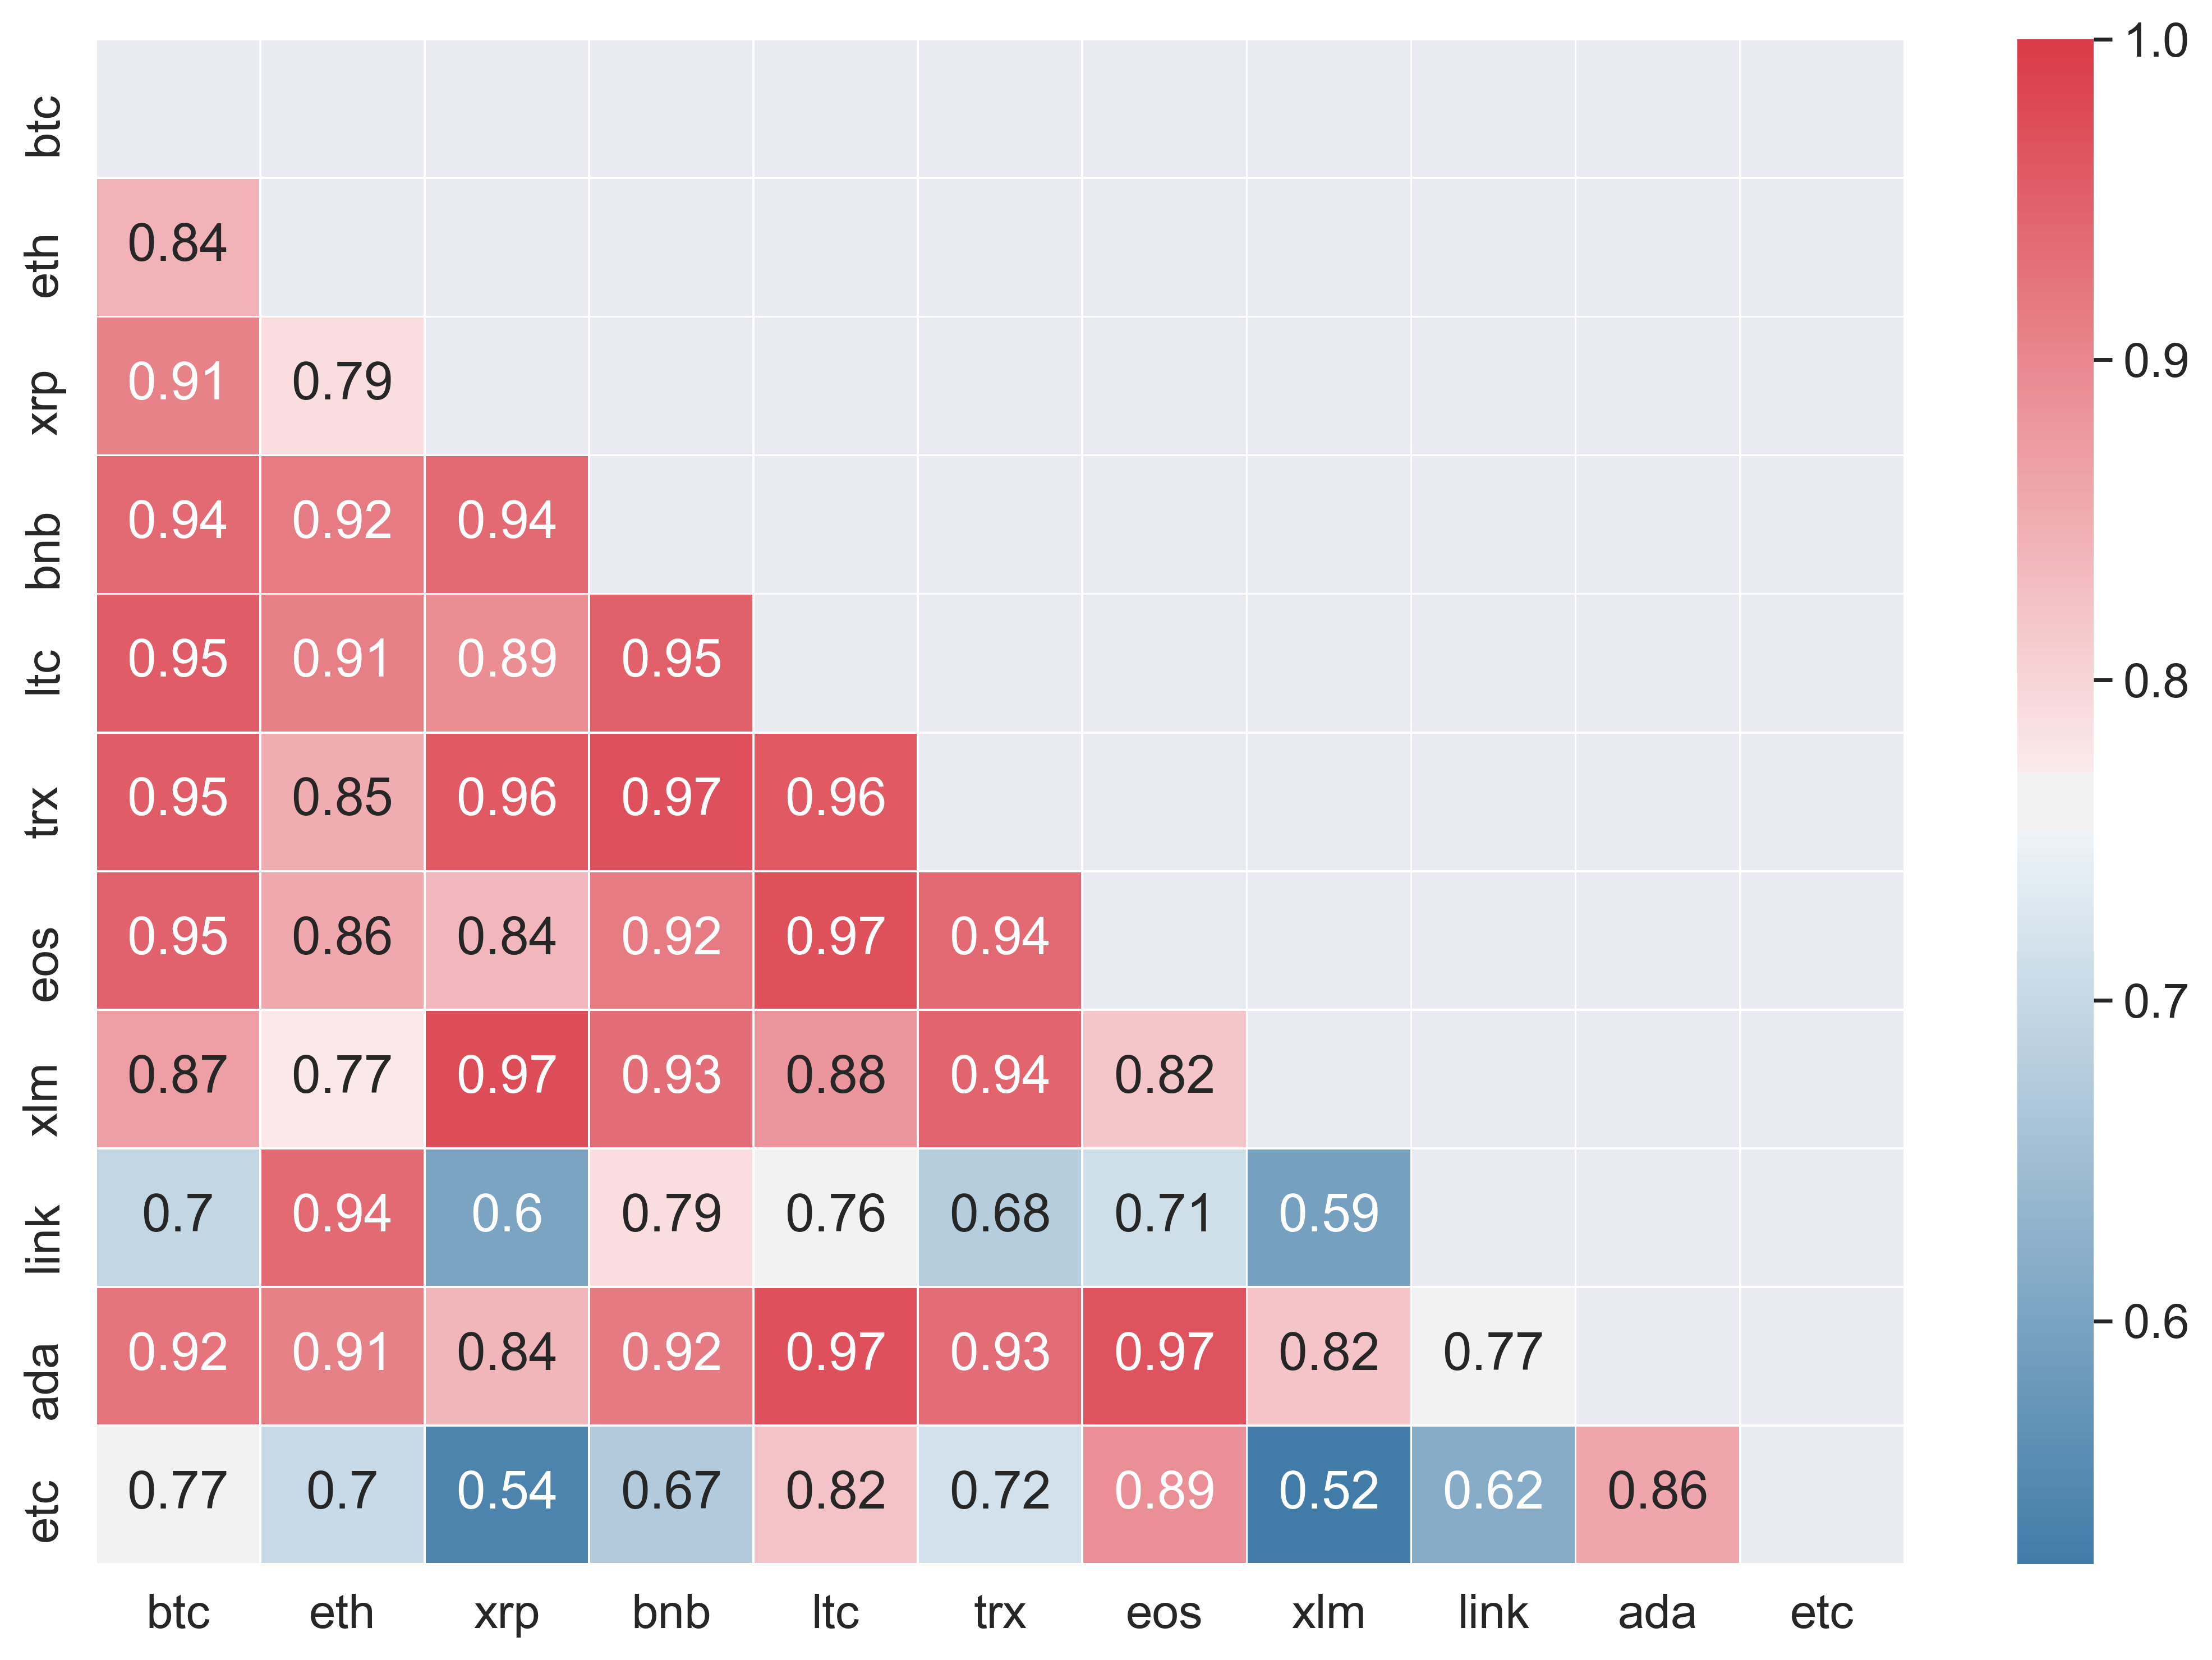
\includegraphics[width=\textwidth,height=\textheight,keepaspectratio]{correlation_heatmap.png}
\end{minipage}
\end{center}

Figure 1 entertains the correlation matrix of the exchange rates in the sample. The exchange rates in the sample are heavily correlated, something that is not often observed in the equity market and FX market. High correlations among assets would be unfavorable for a buy-and-hold strategy, where diversification is desired to rid idiosyncratic risk. However, this does not apply to the market neutral pair trading strategy that is proposed in this paper. The trading system engages in long positions and short positions at the same time and the direction of the market is not the driver of returns. Moreover, high correlations indicate that there are statistical relationships and increase the chance of finding cointegrated pairs of exchange rates. 

% Figure 2
\begin{center}
\begin{minipage}{\textwidth}
\captionof{figure}{Normalised prices over time}
\caption*{\footnotesize The figure shows a comparison of the normalised price series of Bitcoin (BTC), Ethereum (ETH), Ripple (XRP), Litecoin (LTC), EOS (EOS), Binance Coin (BNB), Tezos (XTZ), Stellar (XLM), Cardano (ADA), Chainlink (LINK), Tron (TRX), Monero (XMR), Dash (DASH) and Ethereum Cash (ETC) over the full sample period, from 01-11-2019 00:00 until 29-03-2020 23:59. The exchange rates are denoted in USDT and represent minute-binned data.}
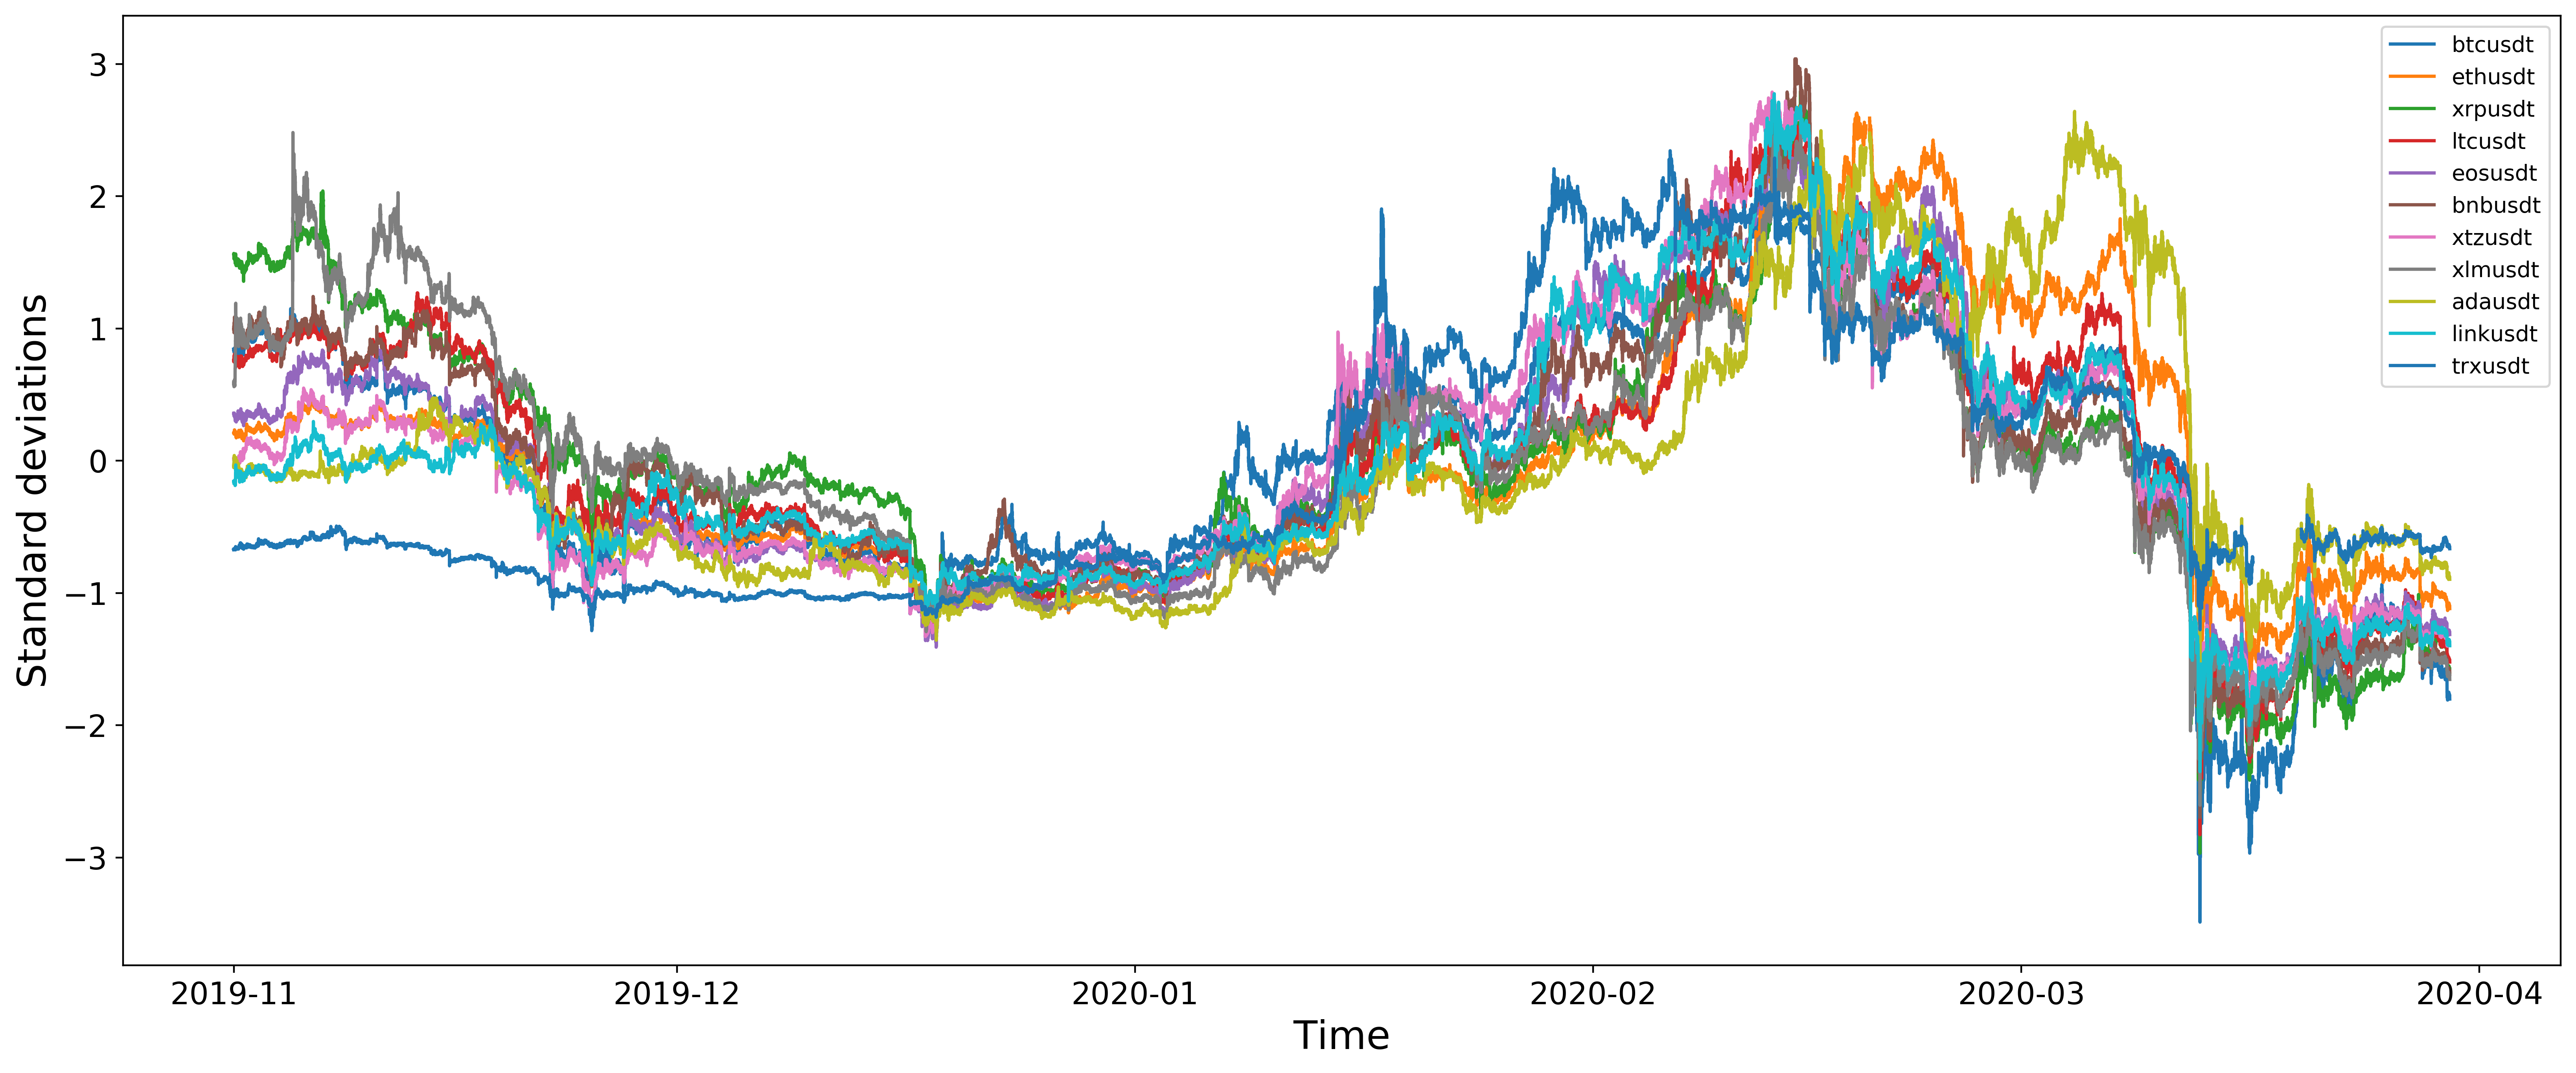
\includegraphics[width=\textwidth,height=\textheight,keepaspectratio]{all_crypto_price_plot.png}
\end{minipage}
\end{center}

Figure 2 shows that the cryptocurrencies in the sample are comoving over a period of five months. The aforementioned volatility is clearly present in the plot. Throughout January, February and March, price levels grow to a high that has only been observed in the last bubble in 2018. With the corona virus spreading in March, the market collapsed, but stabilised later in that month. The expectation is that the volatility gives rise to intraday trading opportunities that would not be observable in daily data. With a larger number of trades with short investment horizons, the proposed high frequency pair trading system is expected to be more profitable compared to a pair trading system that trades on daily data.  

Even though the sample period is short, it covers both calm and stressed periods. This contributes to the robustness of the results, as the performance of the high frequency pair trading system is assessed in a varying set of market scenarios. 

% Table 1: descriptive statistics

\begin{table}[h]
\centering

\caption{\label{tab:table-name} Descriptive statistics}
\caption*{\footnotesize The table shows the descriptive statistics of the minute-binned exchange rates of each cryptocurrency with respect to USDT in the full set ranging from 01-11-2019 00:00 until 29-03-2020 23:59.}

\resizebox{\textwidth}{!}{\begin{tabular}{llllllllllll}
  \Xhline{2.25\arrayrulewidth}
  
\thead{} & \thead{btcusdt} & \thead{ethusdt} & \thead{xrpusdt} & \thead{bnbusdt} & \thead{ltcusdt} & \thead{trxusdt}  & \thead{eosusdt}  & \thead{xlmusdt}  & \thead{linkusdt}  & \thead{adausdt}  & \thead{etcusdt}\\

  \Xhline{0.5\arrayrulewidth}
count&215182&215132&213575&214930&211337&211111&208335&203367&199630&195082&190973\\
totality&99.62\%&99.60\%&98.88\%&99.50\%&97.84\%&97.74\%&96.45\%&94.15\%&92.42\%&90.32\%&88.41\%\\
mean&8093.744&172.601&0.229&17.012&53.719&0.016&3.237&0.058&2.759&0.043&6.671\\
std&1227.671&43.014&0.042&3.752&12.638&0.003&0.810&0.012&0.837&0.011&2.790\\
min&3810.780&86.370&0.106&6.401&24.260&0.007&1.386&0.026&1.386&0.018&3.104\\
max&10500&288.150&0.345&27.176&84.040&0.027&5.495&0.089&4.969&0.072&13.21\\
var&1507175.594&1850.237&0.002&14.078&159.724&0.000&0.657&0.000&0.700&0.000&7.786\\
skew&-0.316&0.854&0.045&0.289&0.391&0.285&0.543&0.121&0.924&0.566&0.713\\
kurt&-0.451&-0.240&-0.370&-0.504&-0.844&-0.299&-0.329&-0.768&-0.346&-0.369&-0.907\\
   \Xhline{1.5\arrayrulewidth}
\end{tabular}}
\end{table} 

Table 1 shows that the price per unit of some cryptocurrencies in USDT is very high. This will not be a problem because Binance allows traders to place orders with quantities with up to eight decimal points. The minimum and maximum prices show that most exchange rates are volatile as the minimum price and maximum price are approximately a factor of 0.5 and 1.5 of the mean price, respectively. Except for Bitcoin (BTC), all exchange rates are unanimously left-skewed and all exchange rates are platykurtic distributed. Further analysis will reveal if the non-normal characteristics play a part in defining trading rules which rely on normality. 


% ############################################################################################################
% Methodology section
\section{Method} \label{sec:Method}

The methodology describes the two stages of the research separately. The first stage describes the statistical models that will be used to identify associated cryptocurrencies by the means of cointegration tests. The tests will be first conducted in the month of the sample first and will yield the initial parameters that can be used in the subsequent stage. In the second stage I will describe how the identified pairs are traded in a high frequency pair trading system by defining some rules.  

There are several approaches to identify associated financial assets. Correlation analysis would not be sufficient because it would run the risk of spurious regression and it would not be possible to conclude that the spread of a pair mean-reverts. Nobel laureates Robert Engle and Clive Granger introduced the concept of cointegration in 1987, which can be used to find time series with a long run relationship \cite{Engle_1987}. This technique is based on regression with integrated regressors. Another approach is introduced by Søren Johansen in 1988 and is based on maximum likelihood estimators and likelihood ratio tests rather than regression \cite{Johansen_1988}. This is deemed a more sophisticated approach towards cointegration because it requires just one step and can identify multiple cointegrated vectors simultaneously. Because cointegration reflects how exchange rates are tied together by a common stochastic trend and quantify the tradable spread, the aforementioned tests are relevant for this paper. Even though both tests are testing the same phenomenon, both tests will be performed to discover any pitfalls \cite{Gonzalo_1998}. The application of the Engle-Granger test will be discussed first, followed by the Johansen test.

\subsection{Engle-Granger} \label{sec:Engle-Granger}

The exchange rates of two cryptocurrencies A and B is represented by a time series $x$ and $y$ as logarithmic prices, respectively. 

$$ x_t = log(p^A_t) $$
$$ y_t = log(p^B_t) $$

The time series are expected to be first-order integrated $I(1)$, so non-stationary. For clarification, a time series is integrated of order $q$ if the time series can be differenced $q$ times to make it stationary, denoted by $I(0)$. In the equity market, this step could potentially be skipped because it is expected that prices take a random walk \cite{Fama_1995}. However, this is not the case in the emerging and still inefficient cryptocurrency market \cite{Urquhart_2016}. To test non-stationarity or integration of the first order, the Augmented Dickey-Fuller (ADF) test with constant and trend will be performed on each time series $i$, where $i \in [1,…,C]$ and $C$ is the number of distinct exchange rates in the sample \cite{Fuller_1979}.

\begin{equation} \label{eq:ADF}
\Delta y_{i, t} = \alpha + \beta_t + \psi_{1, i} y_{i,t-1} + \sum_{j=0}^p \psi_{i, j} \Delta y_{i,t-j} + \epsilon_{i,t}
\end{equation}

$p$ number of lags is estimated by descending iteration starting at $p_{max}$ and by optimising the Akaike Information Criterion (AIC). The ADF test includes lagged terms to rid the effect of autocorrelation. There is a rule of thumb in setting the maximum number of lags, as displayed in equation 2 \cite{Schwert_2002}. Here, $T$ is the number of observations.   

\begin{equation} \label{eq:ADF}
p_{max}= \left[12 \;(T/100)^{1/4}\right]
\end{equation}

The null hypothesis states that $\psi$ in equation 1 is at least one, which would mean that there is a unit root and confirms that the time series is non-stationary. The alternative hypothesis states that $\psi$ is smaller than one, denying the presence of a unit root and assuring stationarity. To check if the null hypothesis can be rejected, the critical values from Mackinnon are used, which account for sample size \cite{Mackinnon_1991}.

If the null hypothesis of the ADF test is not rejected, the time series of prices is found to be $I(1)$, and may proceed to the next step. A linear combination of the two $I(1)$ exchange rates is found through OLS regression. As shown in equation 3, time series $y_{i,t}$ will be regressed on time series $x_{i,t}$ and the residual is tested for stationarity by means of the ADF test. To conclude that a pair is cointegrated, the residual must be stationary. No constant or trend component is included to test stationarity in the residual and, similar to the previous ADF test, the number of lags is chosen by optimising the AIC. If the error term is $I(0)$, it can be concluded that the two time series are cointegrated. This implies that the spread is stationary and that deviations from the equilibrium relationship have finite variance, while the time series contained in the regression are non-stationary and have infinite variance. 

The estimated $\hat{\beta}$ from equation 4 is the hedge ratio in the pair trading strategy and represents the number of cryptocurrency $x$ that need to be shorted or longed for each unit of $y$ that is longed or shorted, respectively. The estimates of the regression can be used to calculate the spread. Because the prices of both assets are known at $t$, the error term can be calculated by rearranging equation 3, resulting in equation 4.

\begin{equation}
    y_{i,t} = \alpha + \beta x_{i,t} + \epsilon_{i,t} \\
\end{equation}

\begin{equation}
\hat{\epsilon_{i,t}} = y_{i,t} - \hat{\alpha}-\hat{\beta}x_{i,t}
\end{equation}

It is possible to combine 11 time series from the sample into $C^{11}_2=55$ combinations for which the hereinbefore described procedure will be executed. This implies that there are 55 hypotheses that call for simultaneous statistical inference. Seong \citeyear{Seong_2009} proposes a useful multiple comparison correction in identifying cointegrating relationships. The high number of hypotheses increase the chance on a type 1 error, hence the interpretation of the probability of obtaining a significant test result needs to be adjusted. To handle this problem, the significance level of 5\% is divided by the number of unit root tests that are performed on the residual of the OLS regressions. Note that rejection of the null implies cointegration in this case. Now, $\alpha/n$ forms the significance level used for rejection of the null hypothesis, where $\alpha$ is the initial significance level and $n$ the number of tests. As a result, it will be more difficult to reject the null, which is justified by the increased probability of obtaining significant results due to multiple tests being performed simultaneously.

\subsection{Johansen} \label{sec:Johansen}

The multivariate counterpart of the Engle-Granger test is the Johansen test, introduced in 1988.  Rather than using regression, Johansen uses maximum likelihood estimators of cointegration vectors, from which a likelihood ratio test is drawn to hypothesise the number of cointegrating relationships. The Johansen test is deemed a more sophisticated approach due the test being able to identify multiple relationships in a single step. Because the model captures short-run and long-run dynamics, the interpretation is different from the Engle-Granger model and hence both models will be used for a more comprehensive understanding of the relationships between the exchange rates in the sample. 

The first step of this test is to consider an autoregressive model, where the dependent variable is regressed on its own lags. In the multivariate extension of the autoregressive model, the vector autoregressive (VAR) model, each variable is regressed on $p$ lags of the other variables and on $p$ lags of its own. In the VAR model, quantities are vectors and coefficients are matrices. A VAR model with $p$ number of lags is generalised in equation 5, where $\Pi_1$ is the coefficient for the first lag of $x$ and $w_t$ is a multivariate Gaussian noise term. The number of $p$ lags is chosen such that the AIC is optimised. 

\begin{equation}
    x_t = \Pi_1x_{t-1} + \sum^{k-1}_{i=1} \Pi_ix_{t-i} + w_t
\end{equation}

From the VAR model in equation 5, a vector error correction model (VECM) is formed by differencing the time series of prices in equation 6. Here, the number of $k$ lags is the same as the number of lags chosen for the VAR model.

\begin{equation}
    \begin{aligned}
        \Delta_{x_t} & = x_{t} - x_{t-1} \\
        \Delta_{x_t} & = \mu +\Pi x_{t-1} + \Gamma_1 \Delta x_{t-1} + \sum^{k-1}_{i=1} \Gamma_i \Delta x_{t-i} + w_t 
    \end{aligned}
\end{equation}

The Johansen test checks for linear combinations of the time series. This is accomplished by eigenvalue decomposition performed on $\Pi$. Remember that $\Pi$ is a matrix, and its rank is represented by $r$. The Johansen test iteratively tests whether $r$ is equal to zero, one, up until $n-1$, where $n$ is the number of time series included in the test. Under the null hypothesis, $r=0$ and under the alternative hypothesis, $r>0$, where the latter implies that there are cointegrating relationships between two or more time series. The decomposition of $\Pi$ yields a set of eigenvectors. The coefficients that form a linear combination are expressed by the largest eigenvector of this set. 

Gonzalo and Lee find that there are differences between the EG test and Johansen test in specific situations. In most situations the Engle-Granger test is more robust, however, both tests need to be performed to identify any pitfalls (Gonzalo and Lee, 1998). In this paper, the Johansen test will be used in a bivariate form to assure cointegration among the exchange rates in the pairs identified by the Engle-Granger test.

The spread is calculated in each time step $t$ as displayed in equation 4. To account for changing relationships of exchange rate pairs, the hedge ratio $\hat{\beta}$ is reestimated every 1440 time steps in a rolling window fashion. 

\subsection{Trading rules} \label{sec:Trading rules}

This section describes the rules that are used by the high frequency pair trading system to trade the spread. A pair trading strategy is market-neutral by nature and implementing a market-neutral strategy involves engaging into long- and short positions simultaneously, through which market risk is immunised \cite{Jacobs_1993}. The profits of the strategy are driven by deviations of the spread, $\hat{\epsilon}_{i,t}$ from equation 4. For a long time, shorting cryptocurrencies was not possible on many of the cryptocurrency exchanges. Luckily, Binance is offering trading on a margin account at the time of evaluating the strategy. 

For convenience, I will define some variables that make up the profit equation. For simplicity, the trading rules are explained for a single cointegrated pair. Hereafter, the framework will be applied to the full set of cointegrated pairs. The description of the rules is inspired by the research of Lin, McCrae and Gulati \citeyear{Lin_2006}. A position is opened at $t_o$ and closed at $t_c$, given that the preset open-conditions and close-condition have been met, respectively. The cointegrated cryptocurrencies that are traded are denoted by $x_1$ and $x_2$. Finally, $N$ denotes the number of units and $P$ the price.
\bigskip

$N_{x_1}(t_o)$ \hspace{10mm} Units of cryptocurrency $x_1$ that are traded when the position is opened \par
$N_{x_2}(t_o)$ \hspace{10mm} Units of cryptocurrency $x_2$ that are traded when the position is opened\par
$P_{x_1}(t_o)$ \hspace{10mm} The price of $x_1$ when the position is opened\par
$P_{x_2}(t_o)$ \hspace{10mm} The price of $x_2$ when the position is opened\par
$P_{x_1}(t_c)$ \hspace{10mm} The price of $x_1$ when the position is closed\par
$P_{x_2}(t_c)$ \hspace{10mm} The price of $x_2$ when the position is closed\par

\bigskip
Because the spread is a stationary process and can either rise above- or drop below its mean, there are two open conditions with a threshold. The mean, in this case, is regarded as the equilibrium. When the spread drops below the equilibrium, the open-condition is met at $t_0$, $x_1$ is overvalued and needs to be shorted while $x_2$ is undervalued and needs to be longed. In equation 4 $\hat{\beta}$ is estimated and determines the units of $x_2$ that need to be longed for each unit of $x_1$ that is shorted. 

\begin{table}[H]

\caption{\label{tab:table-name} Conditions for trading}
\caption*{\footnotesize Table 2 presents three trading conditions that have to be met in order to make a trade. In each timestep $t$, the spread will be calculated. If the new value crosses a boundary set by the trading conditions, a trade will take place as a consequence.}

\begin{tabular*}{\textwidth}{l @{\extracolsep{\fill}} ll}

\Xhline{2.25\arrayrulewidth}

\thead{Condition} & \thead{Description} \\

\Xhline{0.5\arrayrulewidth}

$\epsilon_{t_o} \leq \mu-m\sigma$ & Open-condition 1 (OC1) \\
$\epsilon_{t_o} \geq \mu+m\sigma$ & Open-condition 2 (OC2) \\
$\epsilon_{t_c} = \mu$ & Close condition (CC) \\

\Xhline{1.5\arrayrulewidth}

\end{tabular*}

\end{table}

Table 2 shows the trading conditions, where $\mu$ represents the mean of the spread, $\sigma$ the standard deviation of the spread and $m$ the magnitude of the threshold. There is a trade-off in setting the thresholds that trigger a trade, earlier identified by Rad, Low and Faff \citeyear{Rad_2015}. With a larger threshold, the profit per trade will be higher, but it is less likely that the spread will cross the threshold, effectively allowing fewer trades to be made. The histogram displayed in Figure 3 shows that it is unlikely that the spread deviates more than two standard deviations from the mean. It is expected that the high frequency pair trading system will make trades frequently when the threshold is set to one standard deviation below- and above the mean of the spread. In order to understand the effect of setting the threshold on the performance of the trading system, five trading systems with will be backtested where $m \in [0.5, 0.75, 1, 1.25, 1.5]$. 

% Figure 3
\begin{center}
\begin{minipage}{\textwidth}
\captionof{figure}{Example of the spread process}
\caption*{\footnotesize The left histogram shows the distribution of the spread between the exchange rates ‘BTC-USDT’ and ‘XRP-USDT’, whereas the right histogram shows the spread between the exchange rates ‘ETH-USDT’ and ‘EOS-USDT’. The spread is calculated in the month preceding the backtesting period.}
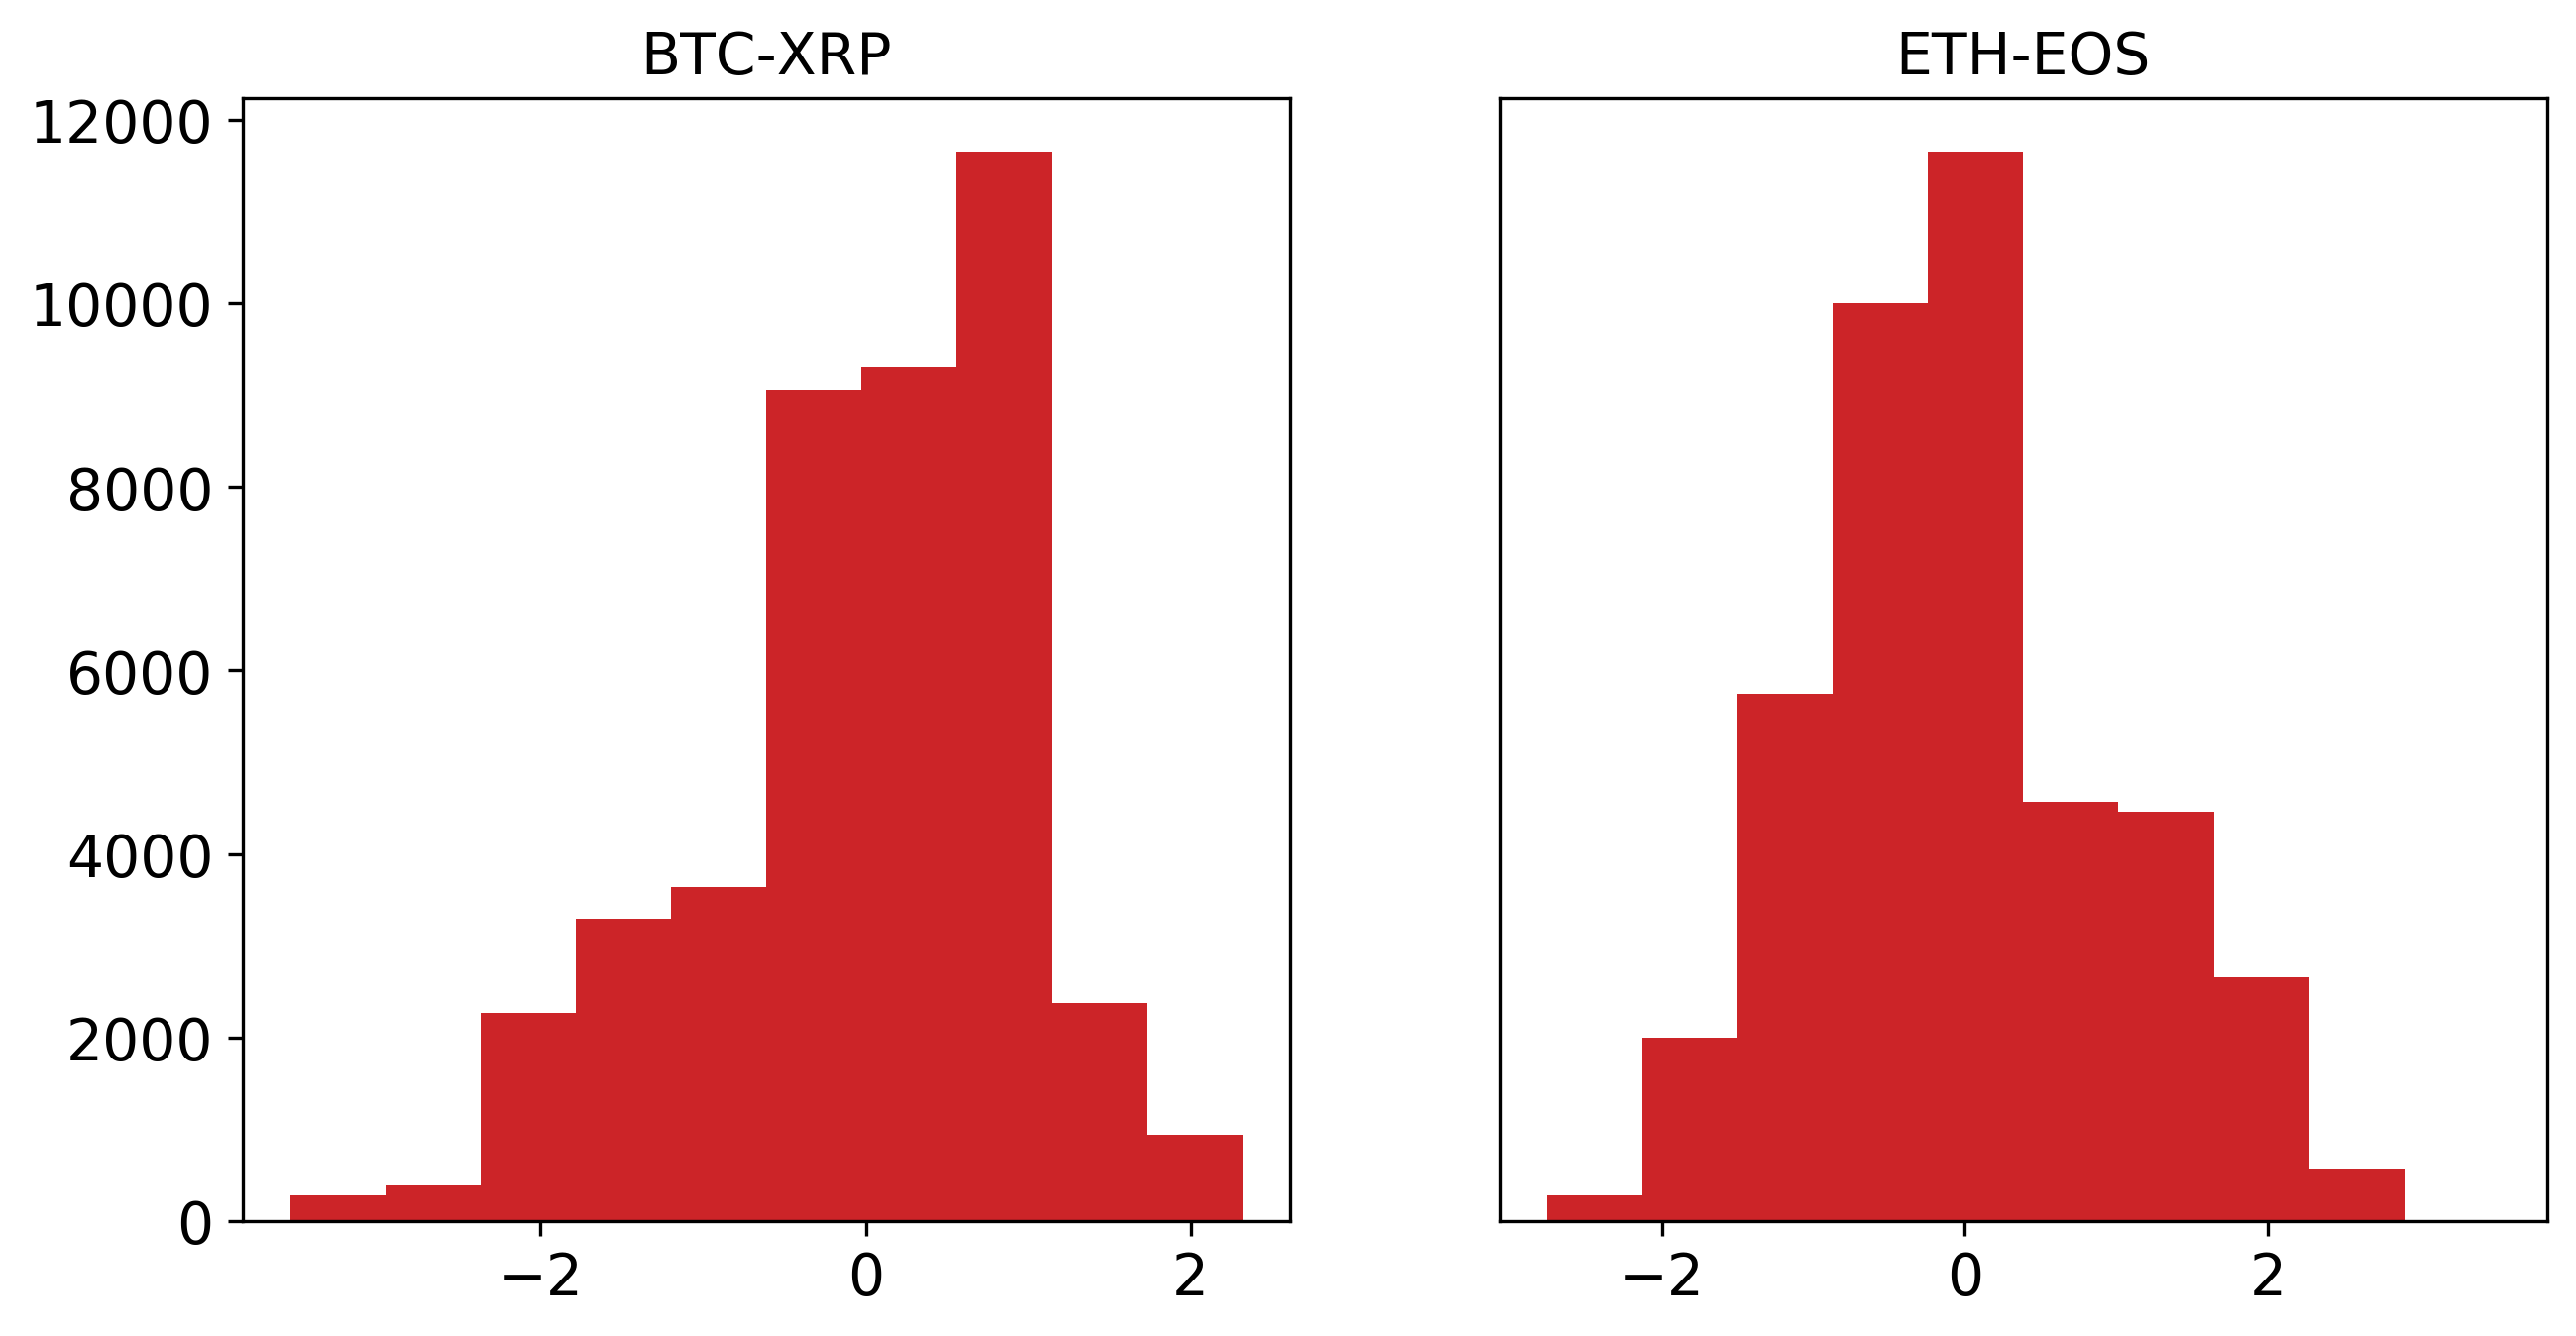
\includegraphics[width=\textwidth,height=\textheight,keepaspectratio]{btcusdt_xrpusdt_spread_hist.png}
\end{minipage}
\end{center}

When open condition 1 (OC1) is met, $x_1$ is overvalued and is shorted such that $N_{x_1}(t_o)$ units are sold for a total of $N_{x_1}(t_o) \; P_{x_1}(t_o)$ USDT. This means that $x_2$ is undervalued and a long position of $N_{x_2}(t_o)$ units is acquired at a cost of $N_{x_2}(t_o) \; P_{x_2}(t_o)$ USDT. When open condition 2 (OC2) is met, $x_1$ is undervalued and $x_2$ is overvalued and as a consequence a short and long position in $x_2$ and $x_1$ are added to the portfolio. Notice that the quantity $N_{x_2}$ is determined by the cointegration coefficient $\hat{\beta}$ from equation 4, so $N_{x_2} = \hat{\beta}N_{x_1}$. Since $\hat{\beta}$ can be a fraction with several decimals, the quantity $N_{x_2}$ is likely to be a fraction too. Luckily, cryptocurrencies can be traded in quantities with eight or more decimals\footnotemark, so it will not be a problem to trade fractions.

\footnotetext{Satoshi Nakamoto decided upon eight decimals because the total bitcoin supply is maxed out at 21 million bitcoins. If the world-wide M1 money supply was divided by the maximum number of bitcoins in circulation, the smallest fraction of a bitcoin (one-eighth) would still be worth less than a penny, making it convenient for people to convert dollars into bitcoin.}

With the prices of either cryptocurrency exchange rate in a pair moving constantly, it is likely that the receipts from a short sale do not fully cover the acquisition of a long position, which means there is some cash outlay. For the implementation of this strategy, a cash amount needs to be invested. I will elaborate on this in the evaluation subsection. With the total receipts of the trades, the profit calculation can be formed as shown in equation 7. The number of units of $x_1$ at open is multiplied by the price of $x_1$ at close minus the price of $x_1$ at open. The same applies to $x_2$ on the right side of $+$ sign. The equation assumes that the $x_1$ is shorted while $x_2$ is longed. 

\begin{equation}
TP_{t_c}=N_{x_1}(t_o)[P_{x_1}(t_c)-P_{x_1}(t_o)]+N_{x_2}(t_o)[P_{x_2}(t_o)-P_{x_2}(t_c)]\\
\end{equation}

Each trade is subject to 0.1\% trading costs on the Binance exchange. To assure a profit with trades that are eligible to transaction fees, the inequality in equation 8 needs to hold. To get transaction fees that are proportional to the total profits of a trade, the receipts of two long positions and two short positions are multiplied by the transaction fee of 0.1\%. Because the trading fee is marginal, it is expected that the transaction fee will not significantly affect the dynamics of the proposed trading system. 

\begin{equation}
    \begin{aligned}
        &TP_{t_c}>b \\
        &b= 0.001 \; [N_{x_1}(t_o) \;P_{x_1}(t_o) + N_{x_2}(t_o) \;P_{x_2}(t_o)]\;+\;0.001 \; [N_{x_1}(t_c) \;P_{x_1}(t_c) + N_{x_2}(t_c) \;P_{x_2}(t_c)] 
    \end{aligned}
\end{equation}

The trading rules thus far rely on the assumption that the pair of cryptocurrencies remain cointegrated. However, sudden price movement from either of the constituents can cause the cointegrating relationship to break. Without cointegration, the spread of the pair is no longer mean-reverting, which disables the trading system to make profitable trades on short-term deviations. Stop-loss orders are commonly used among pair trading practitioners. Miao \citeyear{Miao_2014} uses a stop loss order at 4 standard deviations above and below the mean. Executing stop loss orders is a last resort because the positions are closed at unfavorable prices and thus costs money. Moreover, cryptocurrency exchange rates show volatile behaviour and strong signs of comovement, as displayed before in Figure 2. Due to these observed characteristics, it is expected that the spread processes of cointegrated pairs is volatile, but still mean-reverting. Figure 4 shows an example of a spread process in the first month of the sample. What can be observed is that the spread drops to 5 standard deviations below the mean and consequently mean-reverts. To allow the trading system to profit from these large deviations, the system doesn't incorporate a stop-loss. This is supported by findings from Leung and Nyugen \citeyear{Leung_2018} who find that a pair trading strategy for cryptocurrency markets is most profitable when no stop-loss order is imposed. 

% Figure 4
\begin{center}
\begin{minipage}{\textwidth}
\captionof{figure}{Spread over time of the pair consisting of LTC-USDT and XLM-USDT}
\caption*{\footnotesize The spread of the pair LTC-USDT and XLM-USDT is normalised to emphasize the distance from the mean measured in number of standard deviations. The spread is measured in the first month of the sample, from 01-11-2019 00:00 until 30-11-2019 00:00. The blue dashed line represents the mean, which is zero when it is normalised. The green and red dashed lines represent respectively one and two standard deviations away from the mean.}
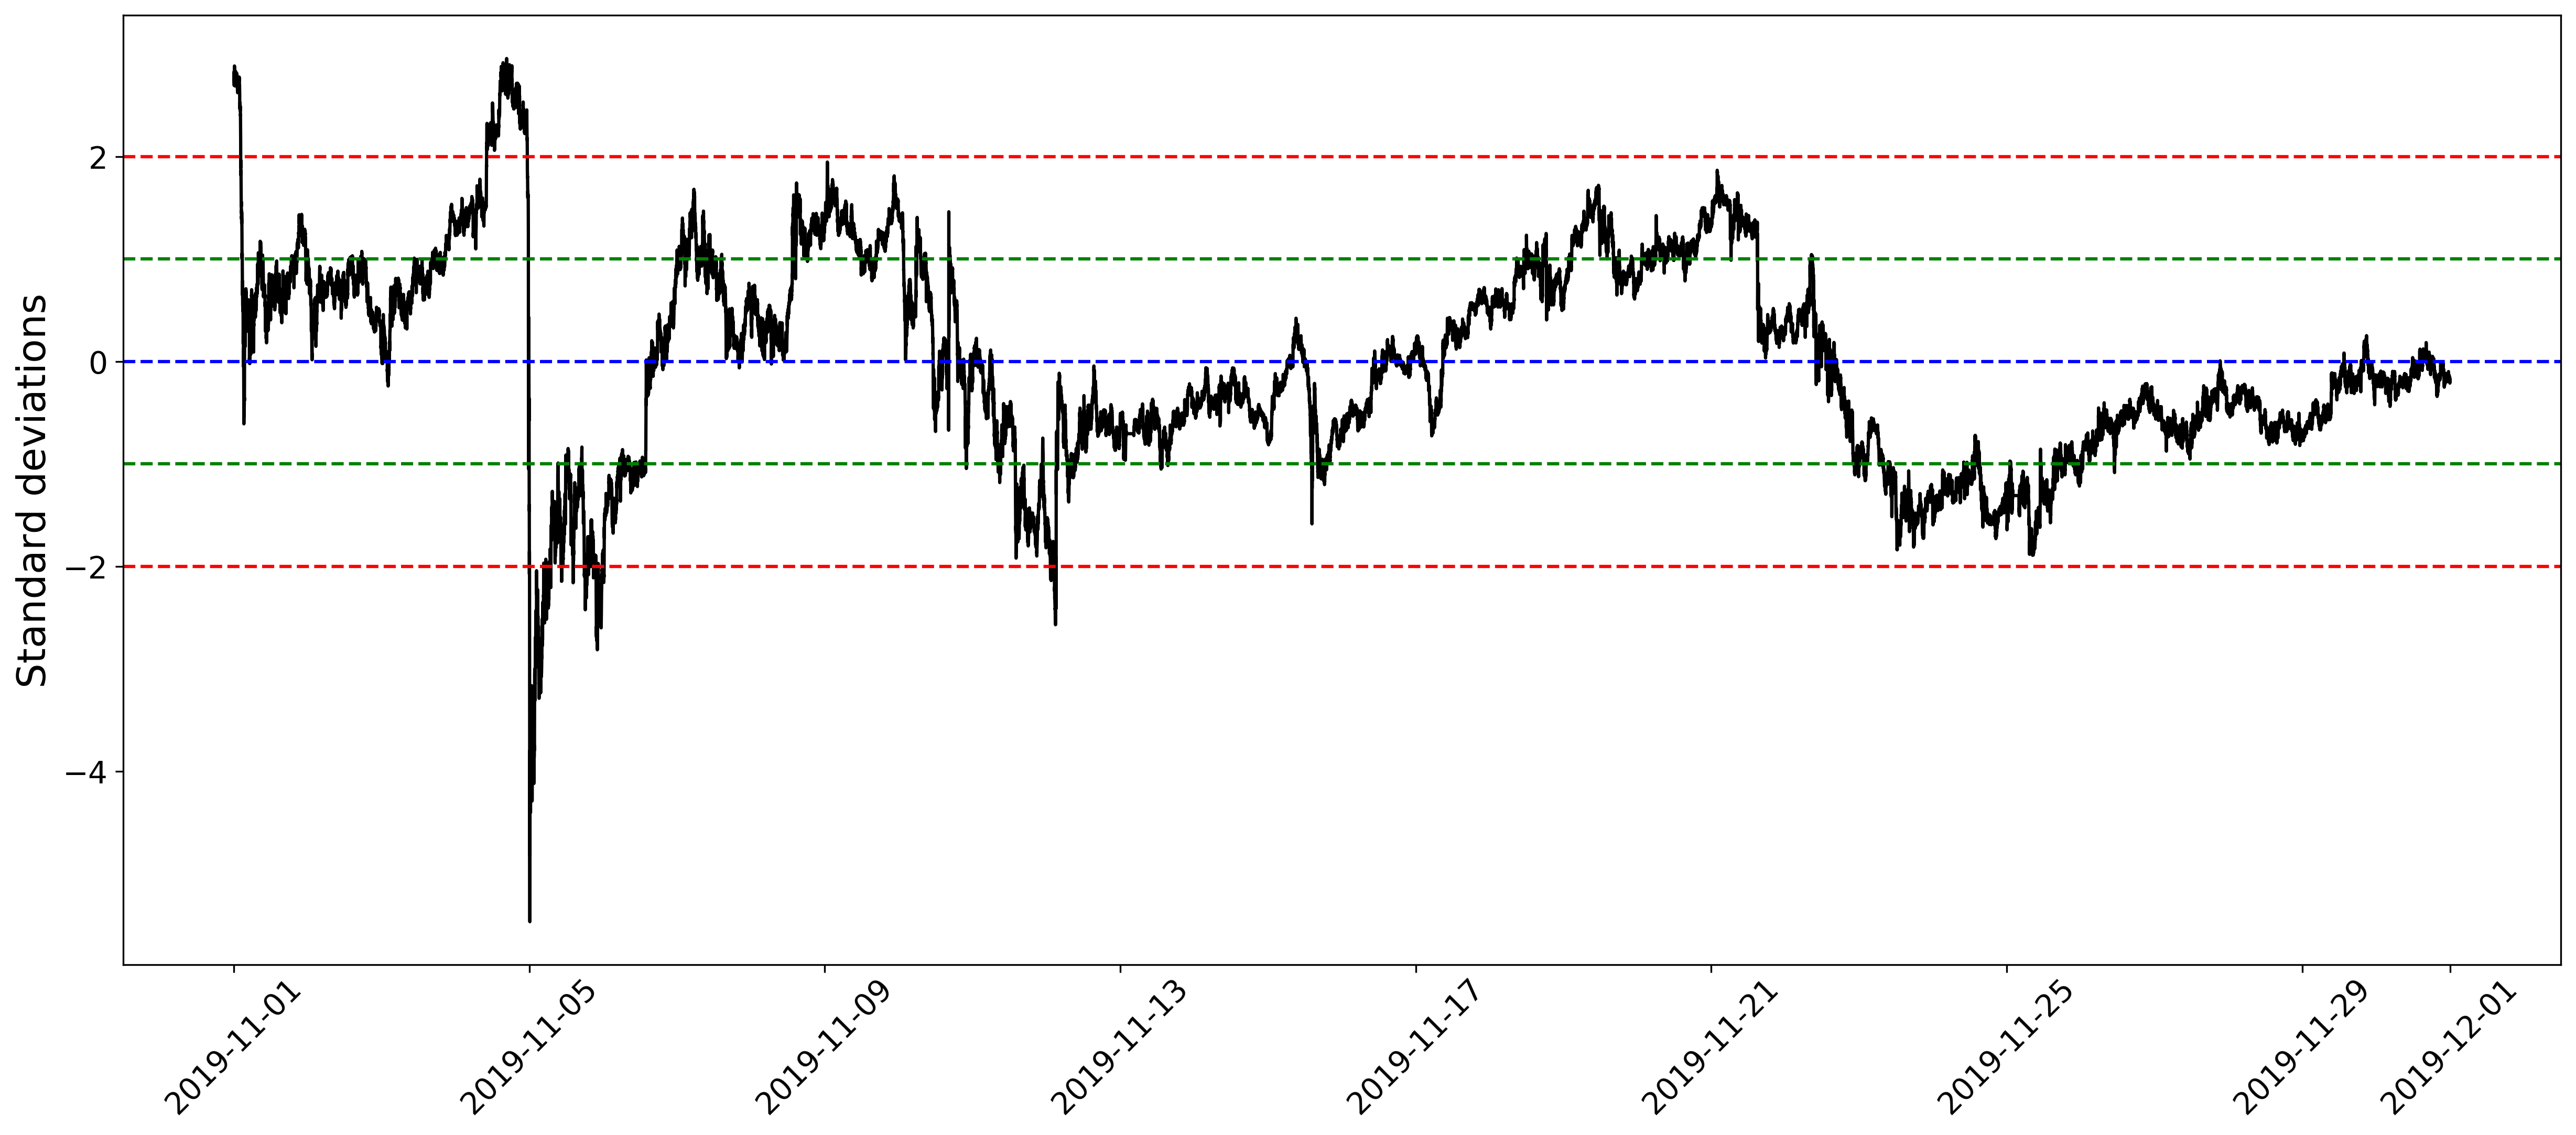
\includegraphics[width=\textwidth,height=\textheight,keepaspectratio]{LTCXLM_spread_process.png}
\end{minipage}
\end{center}

\subsection{Evaluation} \label{sec:Johansen}

The pair trading system that is executing trades based on the hereinbefore described conditions is backtested to evaluate its performance. The pairs that are traded are the pairs that are identified in the first month of the sample and each pair will be allocated 1000 U.S. dollars for the cash outlay that arises from price movements that occur after the last calculation of the cointegration coefficient. The trading system engages in only one trade at the time per pair, which implies that the previously opened long and short position are closed before the next long and short position are opened for the same pair. This construction restricts the amount of cash that is required, because there is no build-up of positions. 

Gatev \citeyear{Gatev2006} suggests two methods to calculate excess returns for a pair trading strategy: the return on committed capital and the return on actual employed capital. In this paper, the return of the portfolio is calculated as the return on committed capital. This is a more conservative way of calculating returns, but is a realistic performance measure for the proposed high frequency pair trading system because the trading system needs to have sufficient liquidity at all times in order not to miss out on trading opportunities. Moreover, long and short positions are marked-to-market at every time step in the backtesting period. 

There are several approaches to measure risk-adjusted return and each approach has its benefits and shortcomings. The Sharpe ratio \cite{Sharpe_1966} scales returns to volatility, where volatility is used to proxy risk. This approach assesses the excess returns per unit of risk and shows if the pair trading strategy truly has an edge on the market or if returns are merely generated by excessive risk taking. 

\begin{equation}
SR = \sqrt{K} {{r_p} \over \sigma_p}
\end{equation}

Equation 9 represents the annual Sharpe ratio, where $r_p$ is the daily excess return, $\sigma_p$ is the standard deviation of daily returns and $K$ equals a constant that relies on the frequency of the data. For daily returns of equity, for example, $K$ equals 252, because there are approximately 252 trading days in one year. In the case of intraday cryptocurrency exchange rates, daily returns and volatility are computed and the Sharpe ratio is calculated on the assumption that cryptocurrencies trade 365 days per year. 

A concern about the Sharpe ratio is raised by Goetzmann, Ingersoll, Spiegel and Welch \citeyear{Goetzmann_2002}, who show that risk-adjusted return is upward biased when the return distribution is not normal, something that is often observed for hedge fund returns. Maximum drawdown (MDD) is an approach to measure risk without assuming a distribution and thus can be used to overcome the limitations posed by the normality assumption of the Sharpe ratio. Rather than taking volatility as a proxy for risk, observed loss patterns over longer periods of time are used. 

\begin{equation}
MDD = {{(P-L)} \over P}
\end{equation}

Equation 10 shows the calculation of MDD, where $P$ is the peak value of the portfolio before the largest drop and $L$ is the lowest value of the portfolio before the highest peak. $P$ and $L$ are measured in the complete backtesting period. To transform this into a comparable risk-adjusted performance measure, return over maximum drawdown (RoMDD) is calculated as displayed by equation 11. 

\begin{equation}
RoMDD = {r_p \over MDD}
\end{equation}

A limitation of RoMDD is that it only measures one dimension of capital preservation and it doesn't say anything about the dynamics of the returns of the portfolio. However, in combination with the Sharpe ratio, it gives insight in the overall risk-adjusted performance of the high frequency pair trading systems with varying thresholds.

% ############################################################################################################
% Results section
\section{Results} \label{sec:Results}

The purpose of this paper is to find long term relationships between cryptocurrency exchange rates with respect to USDT and to trade on short term deviations in order to yield a positive risk-adjusted return. These relationships are found through two distinct cointegration tests, the Engle-Granger test and the Johansen test. The strategy is evaluated as a market neutral pair trading strategy, which means that the performance of the strategy should not rely on the direction of the market. First, I will present the results of the procedures that have been employed to find cointegrated pairs, as described in the methods section. This is followed by the assessment of the performance of the five regimes of pair trading systems with differing opening thresholds in the back testing period from 01-12-2020 00:00 until 29-03-2020 23:59. The performance is evaluated in terms of trade frequency, profit-and-loss (PnL), market neutrality and risk-adjusted return. 

\subsection{Pair selection}

In the first step of the pair formation process the goal is to verify that the price series are $I(1)$. Table 3 shows the results of the ADF test performed on the price series. It can be confirmed that all exchange rates in the first month of the sample are $I(1)$. For an equity portfolio, this step is not necessary because prices in an efficient market are assumed to follow the random walk model \cite{Fama_1995}. This doesn't apply to cryptocurrencies per se, as multiple studies reveal the inefficiency of cryptocurrency markets \cite{Urquhart_2016, Aggarwal_2019}. Nevertheless, all 11 exchange rates can be used in the following steps in which cointegrated pairs are formed for trading. 

\begin{table}[h]
\centering
\caption{\label{tab:table-name} Non-stationarity of cryptocurrency exchange rates with respect to USDT}
\caption*{\footnotesize The cryptocurrency exchange rates in the sample are tested for a unit root by means of the ADF test. The null hypothesis states that the time series in question contains a unit root. The alternative hypothesis rejects the statement that the time series contains a unit root. The null hypothesis is rejected at a 5\% confidence level.}

\resizebox{\textwidth}{!}{\begin{tabular}{llllllllllll}
  \Xhline{2.25\arrayrulewidth}
  
\thead{}&\thead{BTC}&\thead{ETH}&\thead{XRP}&\thead{BNB}&\thead{LTC}&\thead{TRX}&\thead{EOS}&\thead{XLM}&\thead{LIN}&\thead{ADA}&\thead{ETC} \\

\Xhline{0.5\arrayrulewidth}
Test stat.&-2,053&-2,011&-2,923&-1,955&-2,193&-1,856&-2,153&-3,154&-1,566&-2,176&-2,692 \\
P-value&0,572&0,595&0,155&0,626&0,494&0,677&0,516&0,094&0,805&0,503&0,239 \\

\Xhline{1.5\arrayrulewidth}
\end{tabular}}
\end{table} 

Table 4 shows the results of the Engle-Granger procedure and Johansen procedure of the selected pairs of cryptocurrency exchange rates. The results correspond to the month before the backtesting period. Correlation does not belong to the selection criteria but presents a characteristic that is shared among the selected pairs, namely high positive correlation. This implies that the exchange rates move in the same direction. The test statistic is the Dicky-Fuller test statistic and its p-value is calculated by the calculation proposed by Mackinnon \citeyear{Mackinnon_1991}. As opposed to the regular p-value, the Mackinnon p-value takes the sample size into consideration for more accurate inference. This p-value is then subjected to a Bonferroni correction to handle the multiple comparison problem that arises from testing several relationships simultaneously \cite{Bonferroni_1936}. Without such a correction, the probability that a type 1 error occurs is inflated (Seong, 2009). The last column contains the rank of $\Pi$ of the bivariate Johansen test. As the VECM in the Johansen test incorporates short term dynamics, the interpretation may be different from the Engle-Granger test. If the rank equals 1, the test suggests that the pair is cointegrated.

\begin{table}[h]
\centering
\caption{\label{tab:table-name} Pair selection}
\caption*{\footnotesize Eleven cryptocurrency exchange rates with respect to USDT can be combined into fifty-five distinct pairs. Each pair is regressed on one another and the residual is tested for a unit root. The \cite{Mackinnon_1991} p-value corresponds to the augmented dicky-fuller test without constant and trend. The adjusted Mackinnon p-value is corrected with the Bonferroni correction. The last column contains the rank of $\Pi$ of the bivariate version of the Johansen trace test. All tests are performed on the minute-binned exchange rates with respect to USDT in the first month of the sample ranging from 01-11-2019 00:00 until 30-11-2020 23:59. The exchange rates originate from the Binance exchange.}

\resizebox{\textwidth}{!}{\begin{tabular}{llllllllllll}
  \Xhline{2.25\arrayrulewidth}
  
\thead{Pairs}&\thead{Correlation}&\thead{Test statistic}&\thead{Mackinnon p-value}&\thead{Bonferroni p-value}&\thead{Rank } \\

\Xhline{0.5\arrayrulewidth}
LTC-XLM&0.959&-4.952&0.000&0.000&1\\
LTC-EOS&0.994&-4.592&0.000&0.000&1\\
EOS-XLM&0.953&-4.389&0&0.001&1\\
ETH-EOS&0.989&-3.928&0&0.005&1\\
XLM-ETC&0.923&-3.884&0&0.006&1\\
BNB-XLM&0.927&-3.779&0&0.009&1\\
ETH-XLM&0.926&-3.769&0&0.01&1\\
XRP-XLM&0.870&-3.336&0.001&0.048&1\\

\Xhline{1.5\arrayrulewidth}
\end{tabular}}
\end{table} 

A strict selection procedure increases the confidence in the mean-reverting characteristic of the spread of a selected pair. As shown in Table 4, 8 out of 55 pairs have been selected because they meet all the criteria and are concluded to be significantly cointegrated. This meets the expectation that there are significantly cointegrated pairs, substantiated by findings that show interconnectedness in the cryptocurrency market \cite{Ji_2019}, findings that show high correlations among cryptocurrencies \cite{Aslanidis_2019}, as well as the applicability of the Engle-Granger procedure found by Leung and Nguyen \citeyear{Leung_2018}.

\subsection{Backtesting}

The performance of the high frequency pair trading system is evaluated in a backtesting period ranging from 01-12-2020 00:00 until 29-03-2020 23:59. At each timestep $t$ the spread, $\hat{\epsilon_t}$ from equation 4, is calculated and $\hat{\alpha}$ and $\hat{\beta}$ are reestimated in a daily rolling window of one week. The system opens long and short positions simultaneously when $\hat{\epsilon_t}$ hits the thresholds OC1 or OC2, which are reversed when $\hat{\epsilon_t}$ reverts back to the mean, crossing the CC. The portfolio aims to achieve market neutrality by using the cointegration coefficient of a pair to balance out the quantities of the long and short position.

To understand the relationship between the threshold $m$ and the trading dynamics, five regimes of the high frequency pair trading system with varying thresholds are backtested in a period of four months. A comparison of the trading systems is provided in Table 5. As expected, the narrowness of the trading band has a positive relationship with the number of trades executed. The explanation for this is that it is more likely that the spread crosses the thresholds because they require less deviation. Likewise, a trading system with wider trading bands is less likely to execute trades because they require larger deviations. This trade-off was earlier described by Rad, Low and Faff \citeyear{Rad_2015}. 

A shorter holding period is expected to decrease the exposure to price movements that can contaminate the profitability of a trade. An explanation is that the average holding period, $t_c - t_o$, is shorter because the distance between OC1 and CC and OC2 and CC is smaller and thus requires less time to close a position. This expectation is consistent with the findings presented in Table 5, as the share of winning trades increases when the trading band gets narrower.

%SUMMARY TABLE W/O STOP-LOSS
\begin{table}[H]
\caption{\label{tab:table-name} Summary of performance}
\caption*{\footnotesize A summary of the performance of the proposed pair trading system in the backtesting period, from 01-12-2019 00:00 until 29-03-2020 23:59 with varying thresholds. Each trade consists of a long and a short position and its profitability is assessed at closing. PnL stands for 'profit-and-loss'. The final return is based on the cumulative PnL and transaction costs are deducted.}

\begin{tabular*}{\textwidth}{l @{\extracolsep{\fill}} rrrrrr}

\Xhline{2.25\arrayrulewidth}

\thead[l]{Trading system}&\thead{1}&\thead{2}&\thead{3}&\thead{4}&\thead{5}\\
\thead[l]{Threshold}&\thead{\bm{$\pm0.5\sigma$}}&\thead{\bm{$\pm0.75\sigma$}}&\thead{\bm{$\pm \sigma$}}&\thead{\bm{$\pm1.25\sigma$}}&\thead{\bm{$\pm1.5\sigma$}}\\
\Xhline{0.5\arrayrulewidth}
No. winning trades&523&288&281&179&144\\
No. losing trades&138&105&112&74&60\\
Total no. of closed trades&661&393&393&253&204\\
Perc. of winning trades&79.12\%&73.28\%&71.5\%&70.75\%&70.59\%\\
Perc. of losing trades&20.88\%&26.72\%&28.5\%&29.25\%&29.41\%\\
Avg. of winning trades&\$15.00&\$20.28&\$23.45&\$27.01&\$30.13\\
Avg. of Losing trades&\$-48.32&\$-51.72&\$-46.78&\$-59.98&\$-64.88\\
Avg. of all trades&\$1.78&\$1.05&\$3.44&\$1.86&\$2.18\\
Mean daily returns&0.11\%&0.05\%&0.13\%&0.06\%&0.05\%\\
Median daily returns&0.21\%&0.04\%&0.25\%&0.03\%&0.03\%\\
Minimum daily returns&-5.78\%&-5.16\%&-4.13\%&-4.45\%&-4.05\%\\
Maximum daily returns&7.31\%&11.09\%&6.64\%&9.78\%&9.49\%\\
Standard deviation&1.72\%&1.81\%&1.51\%&1.57\%&1.52\%\\
Skewness&-0.05&1.41&0.19&1.72&2.08\\
Kurtosis&3.02&10.72&3.22&11.61&13.44\\
MDD&-29.07\%&-28.73\%&-22.83\%&-24.44\%&-21.07\%\\
RoMDD&1.42&0.59&2.12&0.68&0.8\\
Annual Sharpe&1.26&0.49&1.68&0.71&0.57\\
\Xhline{0.5\arrayrulewidth}
Final PnL&\$1164.02&\$455.88&\$1350.34&\$581.18&\$448.44\\

\Xhline{1.5\arrayrulewidth}
\end{tabular*}
\end{table}

Table 5 shows a positive relationship between the threshold $m$ and the average of winning trades. The profit of a trade can be explained in terms of $\epsilon_{t_c}$ and $\epsilon_{t_o}$. The potential profit increases when the difference between the two terms is large, which is the case when trading with a higher threshold. Interestingly, a similar effect is observed for the average of losing trades, which also increases with the threshold. This indicates that, not only the profit potential increases, but also the loss potential. These findings show the importance of setting optimal thresholds, which can partially be accomplished through backtesting. 

The standard deviation of returns of trading system 3 is the lowest and the mean daily return is the highest, therefore trading system 3 yields the highest annualised Sharpe ratio of 1.68. In the past 10 years, the S\&P500 index yields a Sharpe ratio of 0.84, so the trading system outperforms the market by a considerable margin\footnotemark. Since the Sharpe ratio assumes a normal distribution of returns, its ability to reflect risk-adjusted performance is questionable for trading system 2, 4 and 5. The return over maximum drawdown ratio does not rely on normality of returns, thus complements the Sharpe ratio for a fair comparison. While trading system 5 has the least maximum drawdown, trading system 3 yields the highest return over maximum drawdown (RoMDD). 

\footnotetext{The historical annual Sharpe ratio of the S\&P500 index is measured by Morningstar (www.morningstar.com).}

The objective of this paper is to assess the potential of a high frequency pair trading system to yield a risk-adjusted return, hence, trading system 3 is subjected to more in-depth analysis. From the weekly performance break-down in Table 6 it's possible to draw conclusions about the dynamics of the portfolio relative to the cryptocurrency market and equity market and allows to zoom in on anomalies. 

%NEW TABLE########################################################################################

\begin{table}[ht]
\centering
\caption{\label{tab:table-name} Weekly performance}
\caption*{\footnotesize The performance of the proposed high frequency pair trading system 1 in the backtesting period from 01-12-2019 00:00 until 29-03-2020 23:59 dissected in weeks. From left to right, the week column displays the week in which the performance is measured, followed by the number of observations in that week. The no. of pos. column shows the total number of trades in that week. Each position consists of a long and short position in the exchange rates that compose a pair. The winning trades column shows the number of positions that have been closed with a profit. The average cash flow (CF) column shows the average outlay of cash per position. The profit-and-loss (PnL) column shows the profits per week in U.S. dollars, followed by the best and worst trade in the corresponding week, all denoted in U.S. dollars.}
\resizebox{\textwidth}{!}{\begin{tabular}{lrrrrrrllll}

\Xhline{2.25\arrayrulewidth}

\thead[l]{Week}&\thead{Count}&\thead{No. of pos.}&\thead{No. of closed}&\thead{No. of succes}&\thead{\% Succes}&\thead{Avg. CF}&\thead{PnL}&\thead{Cum. PnL}&\thead{Best}&\thead{Worst}\\

\Xhline{0.5\arrayrulewidth}

48&1440&10&2&2&100\%&\$48.68&\$37.78&\$37.78&\$21.47&\$0.00\\
49&10080&137&70&66&94.29\%&\$151.94&\$596.40&\$634.18&\$24.61&\$-12.19\\
50&10080&37&18&13&72.22\%&\$315.33&\$19.3&\$653.48&\$25.27&\$-38.69\\
51&10080&69&34&31&91.18\%&\$-452.70&\$-66.17&\$587.31&\$49.53&\$-251.14\\
52&10080&50&24&22&91.67\%&\$358.30&\$381.0&\$968.31&\$66.31&\$-47.77\\
1&10800&28&14&13&92.86\%&\$276.81&\$72.61&\$1040.92&\$27.01&\$-24.49\\
2&10080&76&38&30&78.95\%&\$124.43&\$242.69&\$1283.61&\$27.88&\$-114.45\\
3&10080&69&34&20&58.82\%&\$-331.16&\$-443.57&\$840.04&\$39.46&\$-241.05\\
4&10080&32&18&9&50.00\%&\$-193.94&\$-436.32&\$403.72&\$29.24&\$-288.22\\
5&10080&31&14&8&57.14\%&\$249.20&\$-266.76&\$136.96&\$37.39&\$-101.74\\
6&10080&34&17&10&58.82\%&\$-88.51&\$-195.97&\$-59.01&\$33.56&\$-110.34\\
7&10080&52&26&17&65.38\%&\$105.20&\$-346.66&\$-405.67&\$91.35&\$-311.88\\
8&10080&26&15&11&73.33\%&\$66.80&\$-23.31&\$-428.98&\$53.43&\$-233.93\\
9&10080&23&11&6&54.55\%&\$-229.33&\$-94.5&\$-523.48&\$34.50&\$-46.58\\
10&10080&9&4&2&50.00\%&\$43.33&\$30.40&\$-493.08&\$37.48&\$-26.00\\
11&10080&53&27&24&88.89\%&\$-166.06&\$1148.83&\$655.75&\$237.08&\$-177.59\\
12&10080&39&19&15&78.95\%&\$-27.99&\$476.34&\$1132.09&\$107.68&\$-59.50\\
13&10080&19&9&6&66.67\%&\$241.43&\$218.25&\$1350.34&\$102.68&\$-26.68\\
\Xhline{1.5\arrayrulewidth}
\end{tabular}}
\end{table}

Table 6 doesn't show a sound relationship between the number of closed trades and the PnL. For example, week 1 and week 5 have the same number of closed trades while the profits in those week are roughly \$73 and \$-267, respectively. A small number of trades took place in the first week, partially attributable to the fact that the first week consists of only one day. In the following week, the high frequency pair trading system closed 70 trades with an all time high success rate. Profits are growing later in 2019 and in the first two weeks of 2020, after which the trading system is generating significant losses during weeks 3 through 7. The losses in these particular weeks call for further analysis. Figure 5 shows that a shock affected the exchange rates at the end of week 3. From there on, exchange rates drifted apart and the cointegrating relationships were likely to have changed in an unexpected manner, causing the trading system to close positions with a loss. The column with the worst trades indicates that losses are not clustered in individual trades, which implies that the trading system is making several unsuccessful trades as a consequence of dissolving cointegrating relationships of pairs.

Moreover, the average investment is relatively high, indicating that there is a mismatch in capital allocation. Ideally, the receipts of a short position would cover the acquisition of the long position. In the real world, there will always be a mismatch, because prices of assets are moving continuously throughout time. However, a relatively large mismatch can indicate that the relationship between the exchange rates in a pair is changing and that anticipated mean-reversion is not certain.  

% Figure 5
\begin{center}
\begin{minipage}{\textwidth}
\captionof{figure}{Exchange rates in weeks 3 through 7}
\caption*{\footnotesize The weeks correspond to the dates 13-01-2020 until 16-02-2020. The exchange rates of the cryptocurrencies with respect to USDT are normalized in order to make them comparable.}
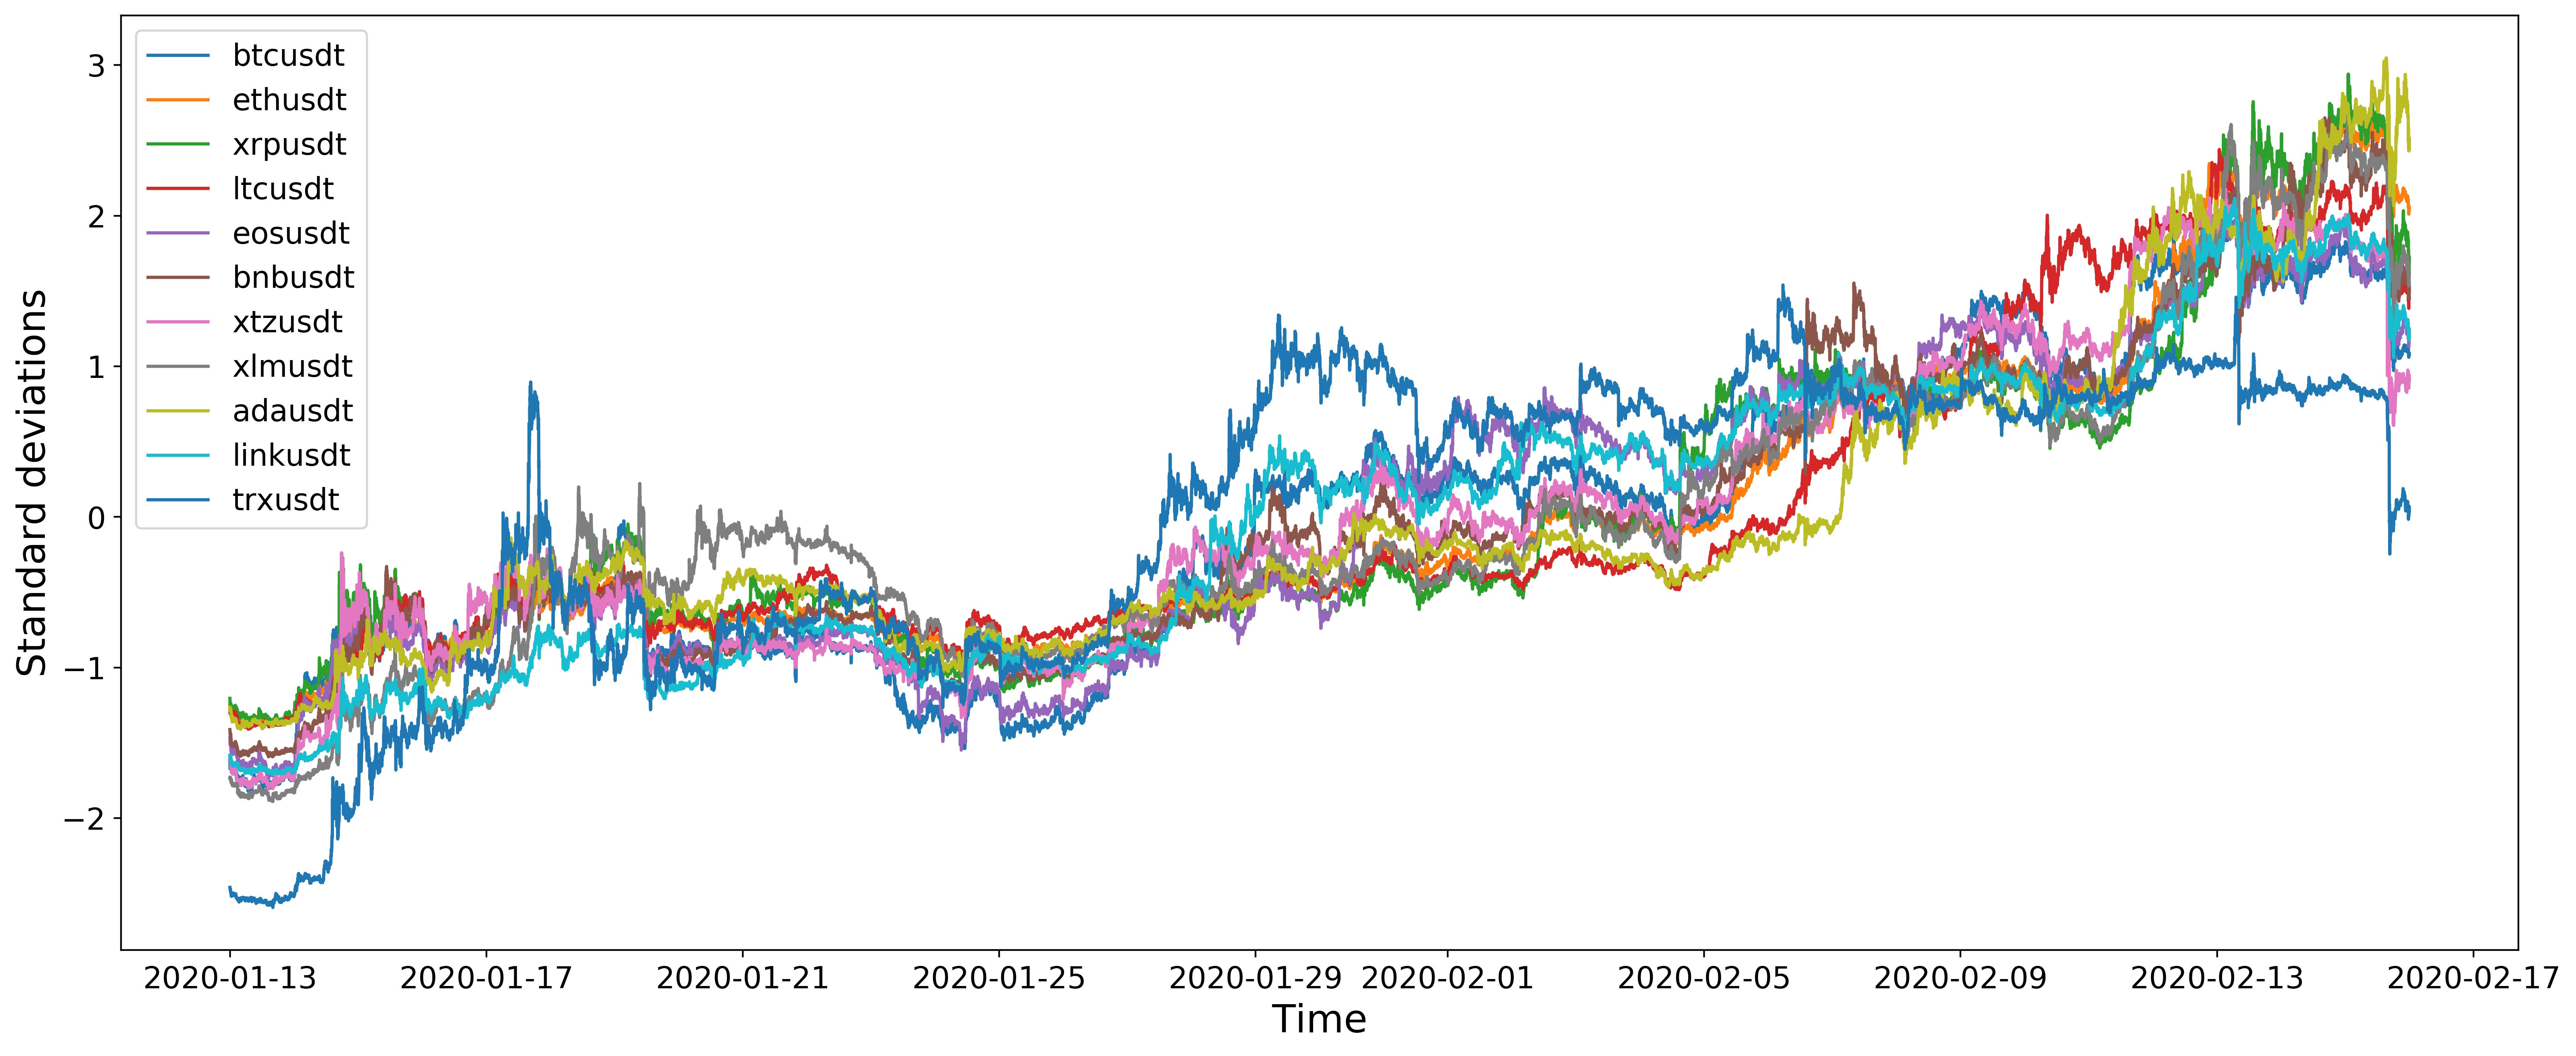
\includegraphics[width=\textwidth,height=\textheight,keepaspectratio]{prices_week34567.png}
\end{minipage}
\end{center}

A notably large profit was made in week 11. This is not attributable to a single trade, as the best trade explains just $1\over5$ of the total profit in the corresponding week. Figure 6 shows that the exchange rates took a big dive towards the end of week 11. Interestingly, all exchange rates followed this pattern, implying that the shock had uniform effect on the exchange rates, which is in congruence with the volatility spillover effect and interconnectedness found in cryptocurrency markets \cite{Ji_2019}. This also indicates that cryptocurrency exchange rates do not offer diversification benefits in order to hedge against shocks within the cryptocurrency market. The high frequency pair trading system is especially making profits when the cryptocurrency market is in downturn. This was also found by \cite{Miao_2014}, who applied a high frequency pair trading system in the equity market. 

% Figure 6
\begin{center}
\begin{minipage}{\textwidth}
\captionof{figure}{Exchange rates in weeks 10 and 11}
\caption*{\footnotesize Weeks 10 and 11 correspond to the dates 01-03-2020 until 14-03-2020. The exchange rates are normalized in order to make them comparable, just for visualization purposes.}
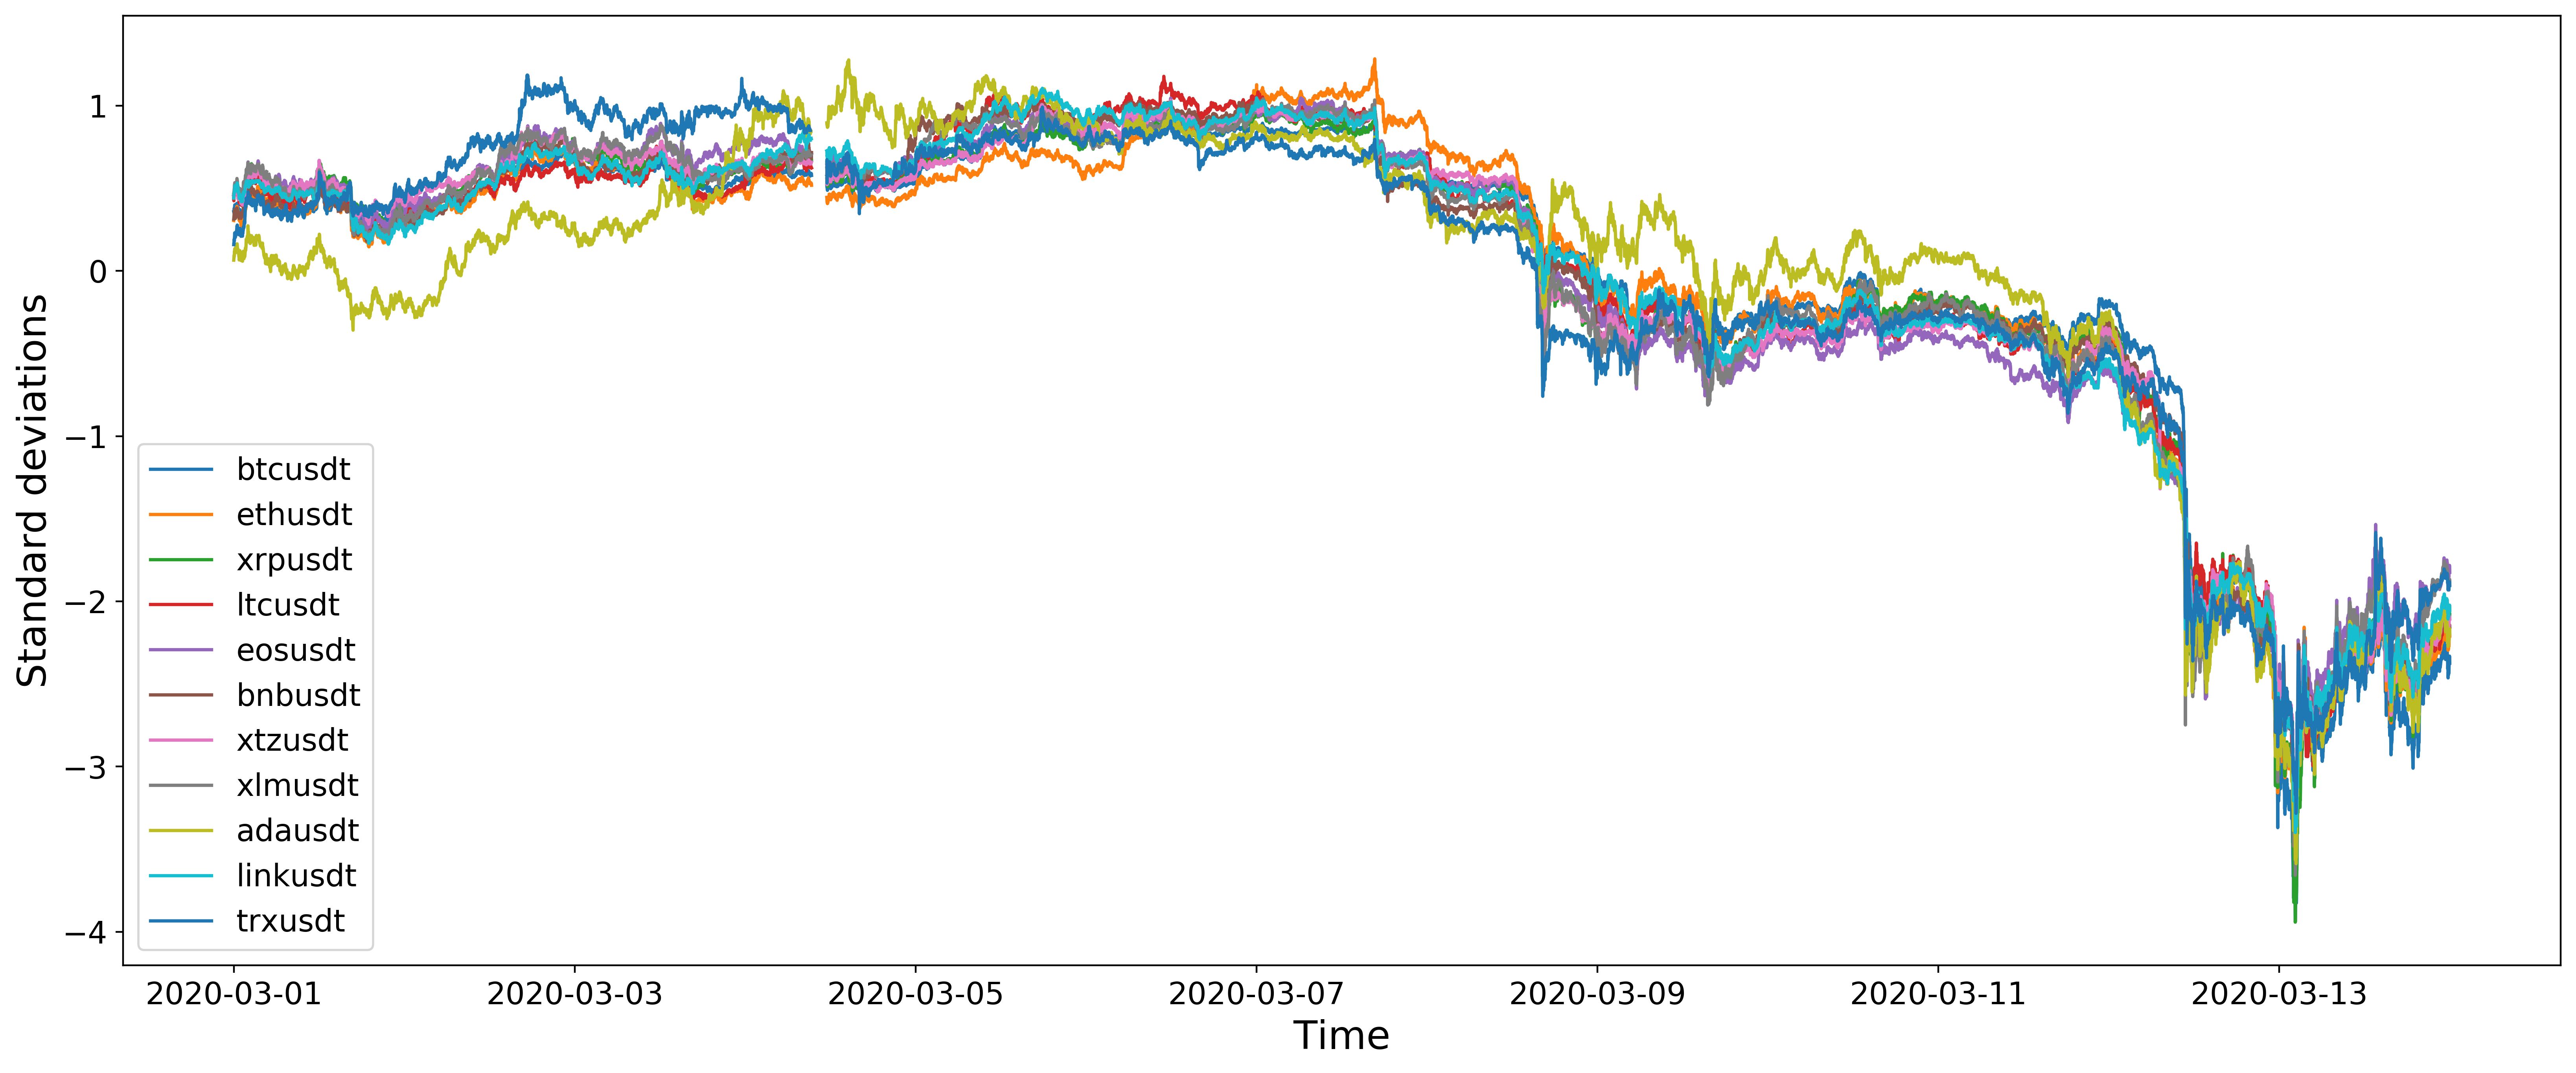
\includegraphics[width=\textwidth,height=\textheight,keepaspectratio]{prices_week1011.png}
\end{minipage}
\end{center}

In Figure 7, the portfolio returns are compared with the returns of the three cryptocurrencies with the highest market capitalization at the time of testing and serve as a proxy for cryptocurrency market returns. This provides an opportunity to assess the degree of market neutrality of the high frequency pair trading system with respect to the market it is trading in. At the start of the backtesting period, the trading system gradually made small profits but got nullified by much larger losses throughout January, also observed in week 4 of Table 6. The winning trades continue to be overshadowed by the losing trades at the start of February. In the period when the portfolio returns are declining, the best trades are much smaller in magnitude compared to the worst trades. The contrary is observed for the frequency, where successfully closed trades still have the majority by a considerable margin. This implies that the trades that yield a profit are dominated by a few bad trades that generate relatively large losses, which might be attributable to the volatility in the exchange rates during that period. Price movements during the holding period can marginalise the profitability of one of the sides of the trade, which contaminates the profitability of the complete position. The exchange rates that are driven apart after the shock, shown in Figure 7, are a real life example of the volatility persistence found by Aggarwal \citeyear{Aggarwal_2019} and serve as an example of the inefficiency in the market found by \cite{Urquhart_2016}.   

% Figure 7
\begin{center}
\begin{minipage}{\textwidth}
\captionof{figure}{Portfolio returns compared to market returns}
\caption*{\footnotesize In the top plot, the cumulative returns of the portfolio are plotted over the backtesting period, from 01-12-2020 00:00 until 29-03-2020 23:59. In the bottom plot, the cumulative returns of the three biggest cryptocurrencies in terms of market capitalization in the pair trading portfolio are plotted over the same period.}
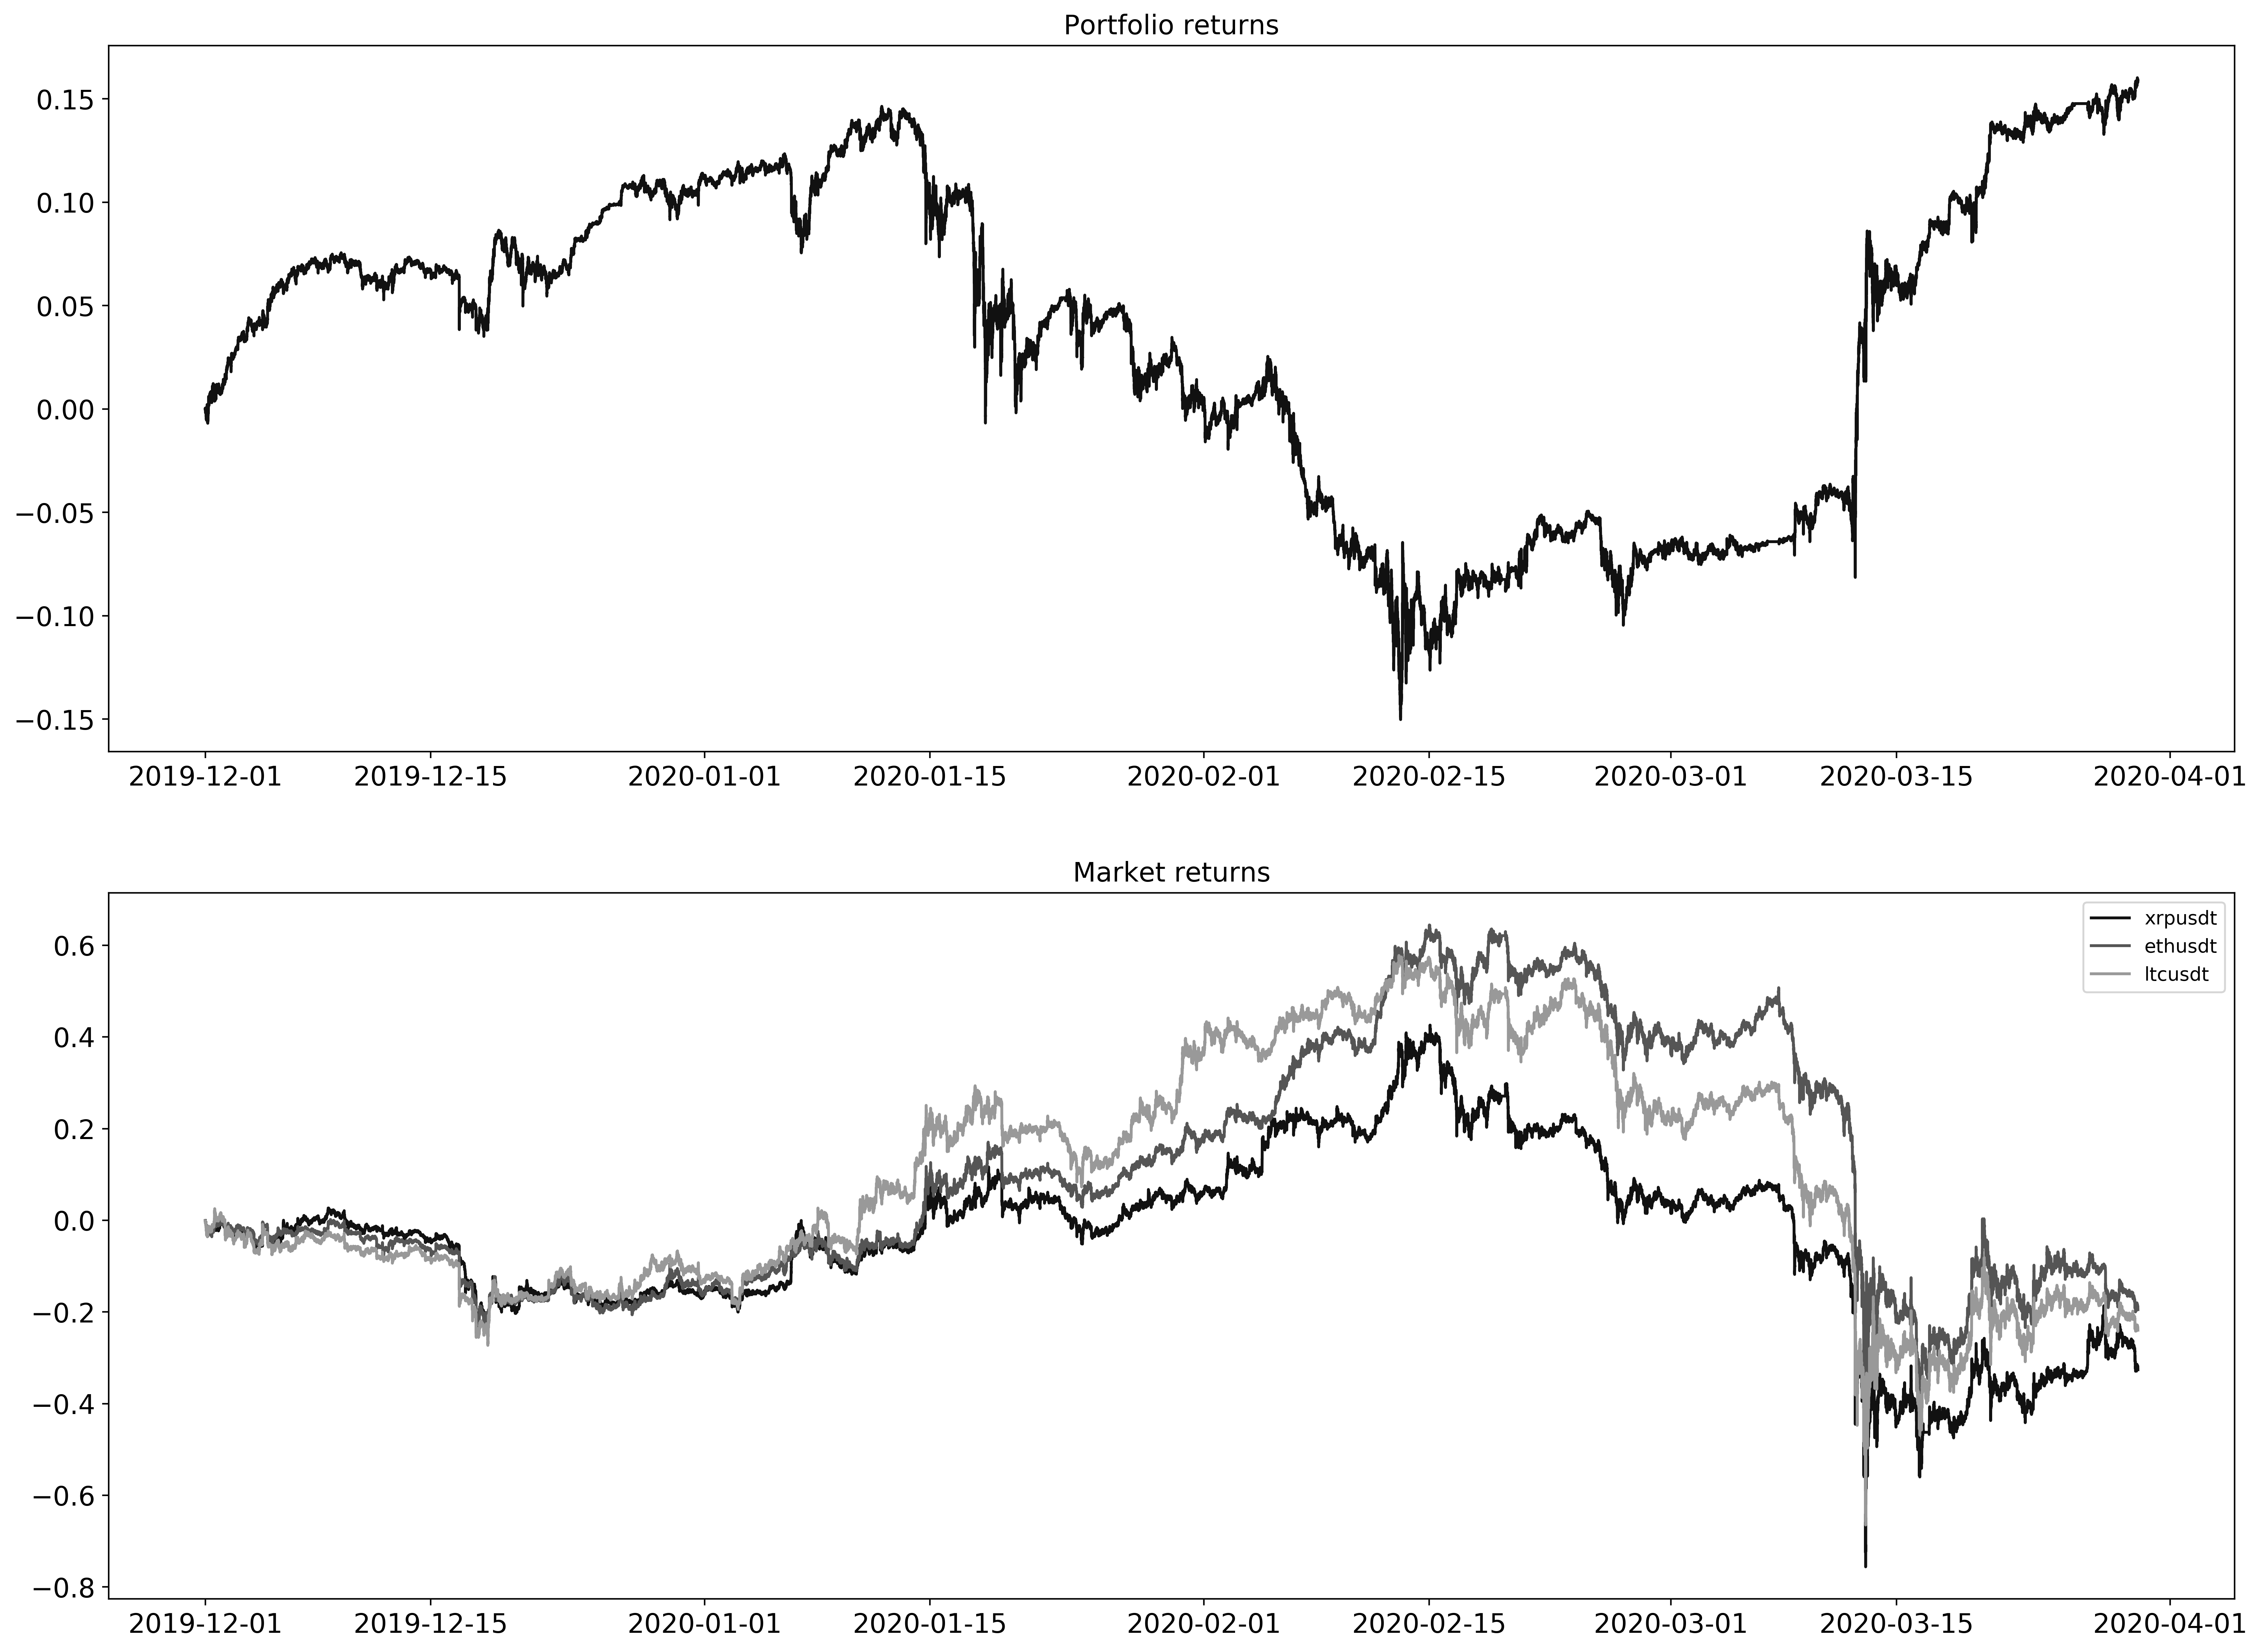
\includegraphics[width=\textwidth,height=\textheight,keepaspectratio]{portfolio_returns_vs_market.png}
\end{minipage}
\end{center}

In week 11, from the 9th of March until the 15th of March, the portfolio returns are notably high, to such an extent that it virtually recovered the losses made before. Figure 7 shows that the market crashes and is making losses as much as 60\%, relative to the start of the backtesting period. Table 6 shows that many trades took place in the week 11, relative to the adjacent weeks, implying that the spread crossed the opening conditions and closing condition several times within a small time frame, yielding significant profits. This is also confirmed by the portion of successfully closed trades, which is 89\% in week 11. The findings show that the trading system captures the mean-reverting characteristics well in a bear market. After the crash, the market is recovering in the second half of March and the trading system is making significant gains, demonstrating market neutrality to a certain extent. 

% Figure 8
\begin{center}
\begin{minipage}{\textwidth}
\captionof{figure}{Portfolio returns compared to S\&P500 returns}
\caption*{\footnotesize The black line represents the cumulative portfolio returns of the high frequency pair trading system. The blue dashed line represents the cumulative return of the S\&P500 index. The left y-axis corresponds to the portfolio returns whereas the right y-axis corresponds to the S\&P500 index returns.}
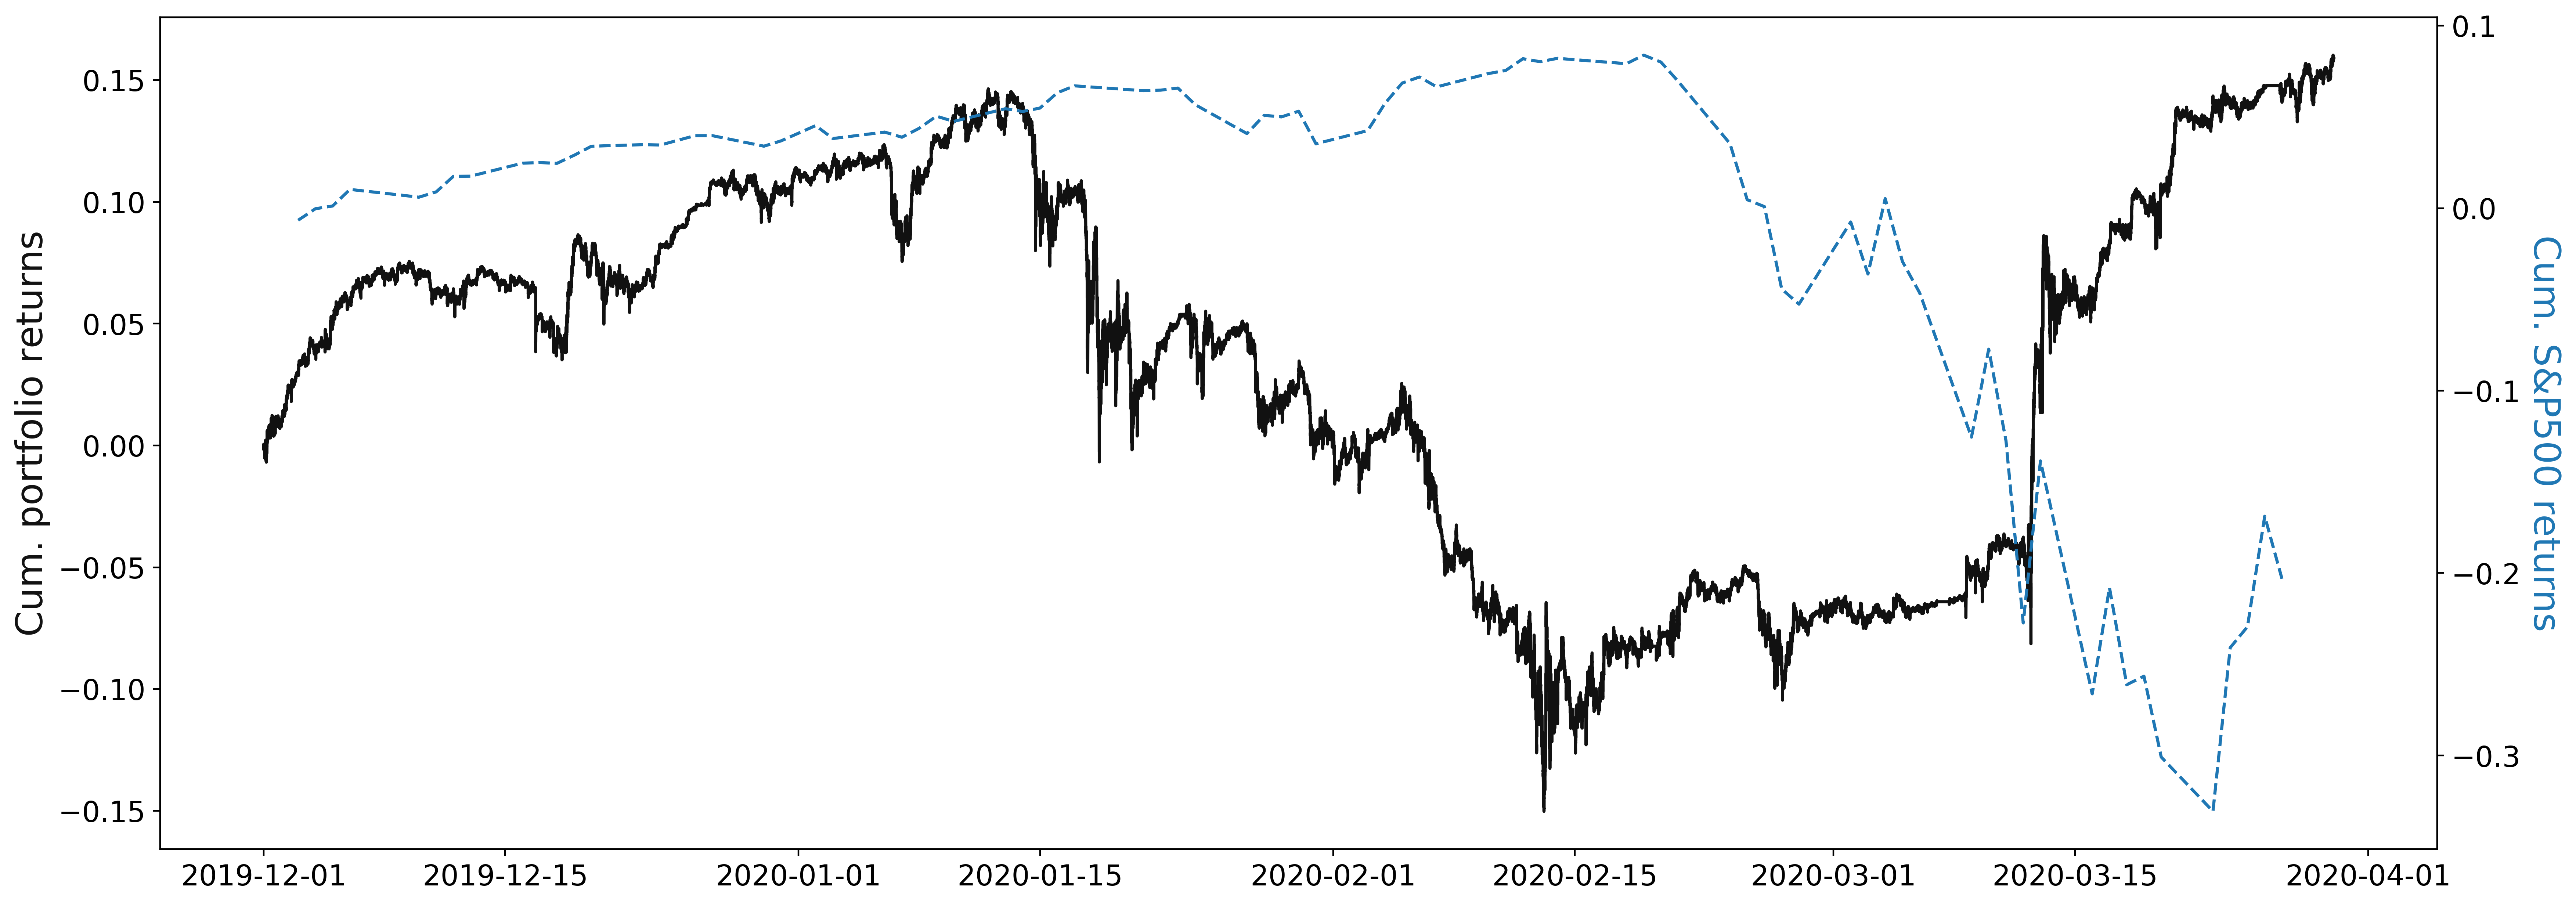
\includegraphics[width=\textwidth,height=\textheight,keepaspectratio]{SP500_vs_PF.png}
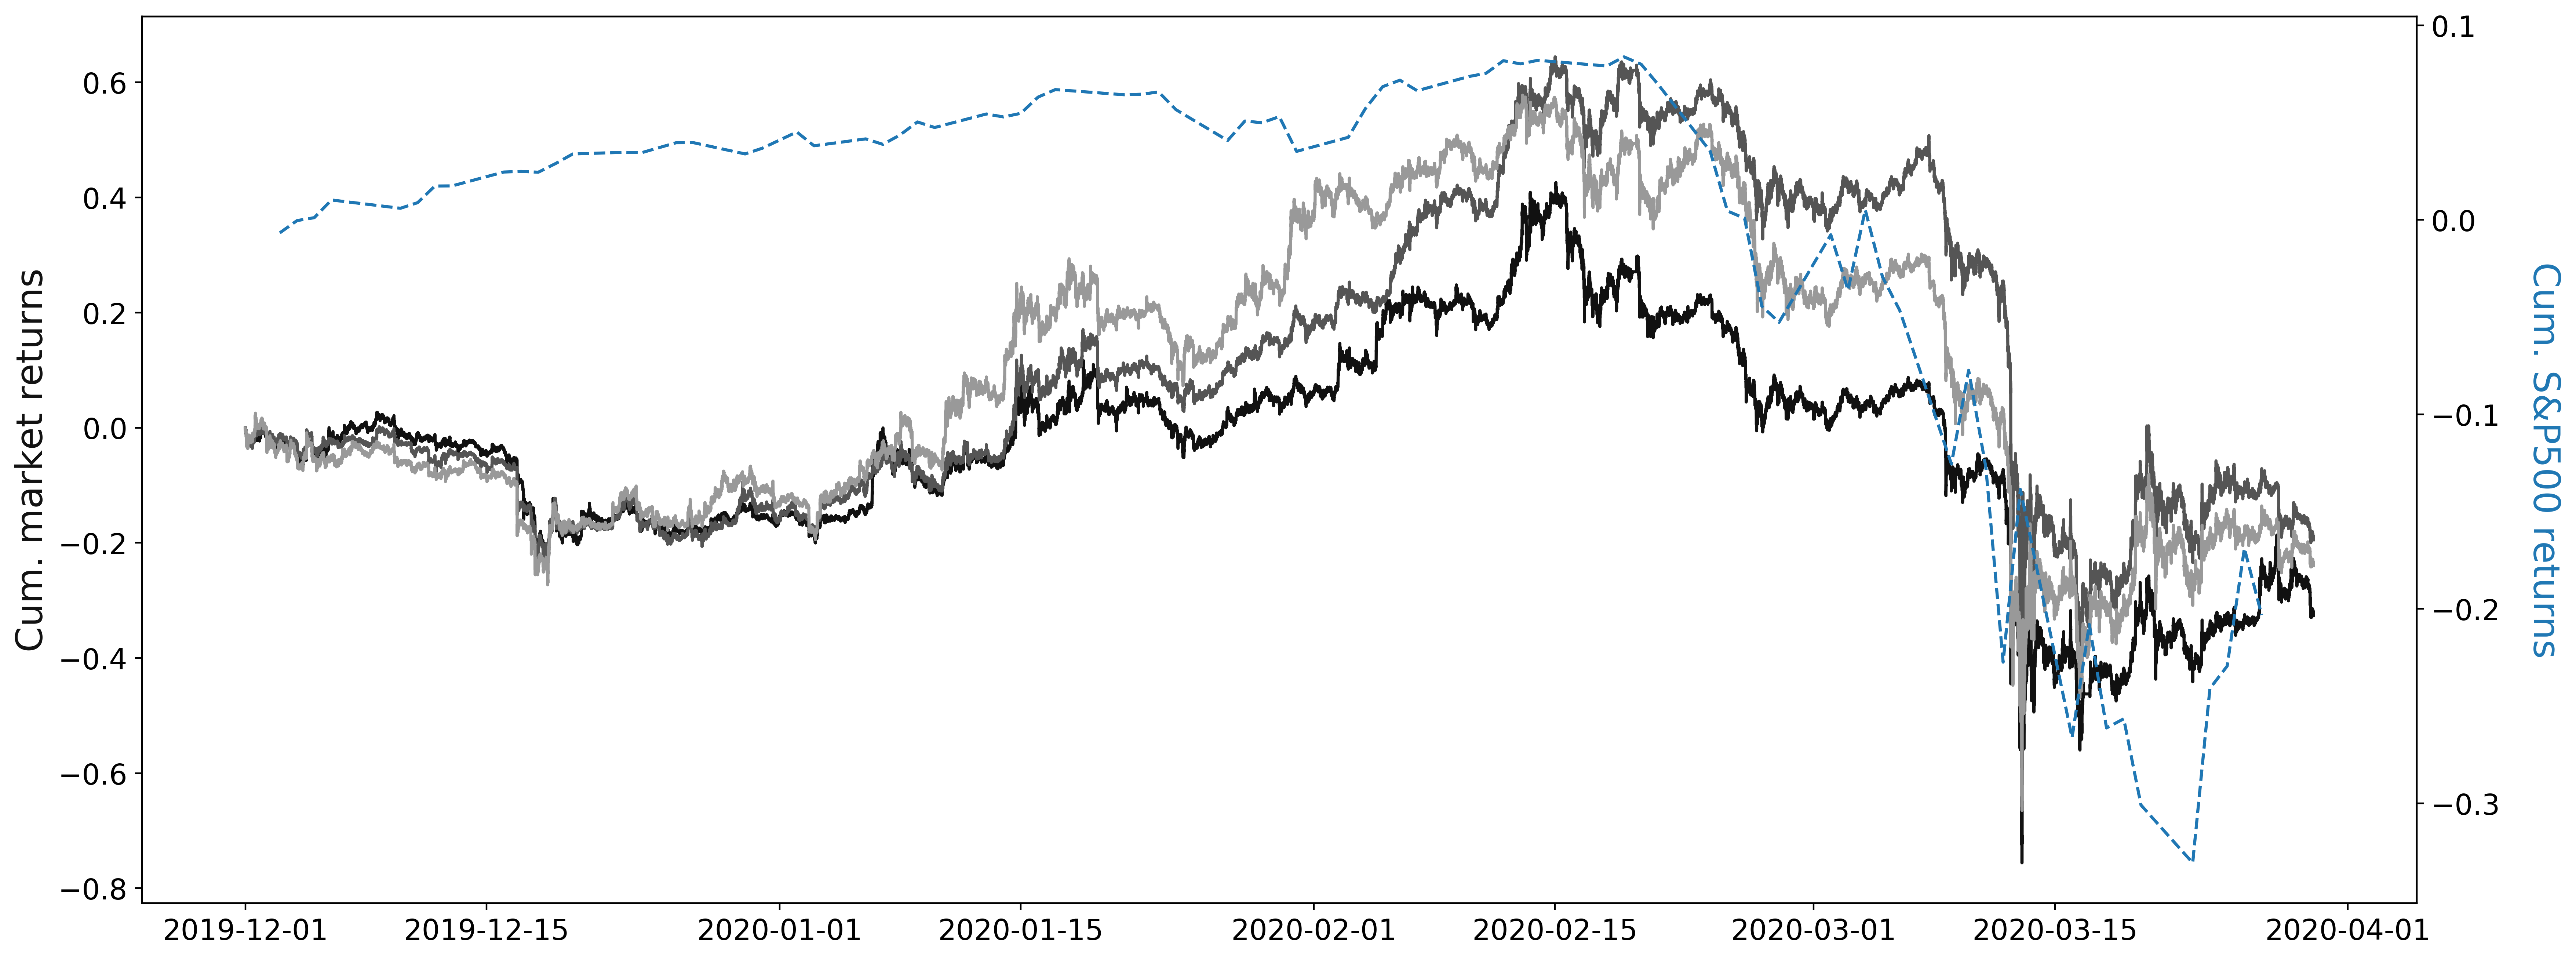
\includegraphics[width=\textwidth,height=\textheight,keepaspectratio]{market_vs_sp500.png}
\end{minipage}
\end{center}

To study potential diversification benefits of the high frequency pair trading system for equity investors and a degree of market neutrality, the portfolio returns are compared with equity market returns, proxied by the Standard \& Poor's 500 (S\&P500) index returns. Earlier research found diversification benefits in the cryptocurrency market for equity investors but noted that cryptocurrencies come with their own hard-to-measure idiosyncratic risk \cite{Corbet_2018}. Risk associated with cryptocurrencies is emphasized by Matkovskyy and Jalan \citeyear{Matkovskyy_2019}, who found contagion effects of financial markets to cryptocurrency markets. In crisis periods, investors move away from risky assets towards safer investments available in the financial market. This implies that there is a clear connection between the equity market and the cryptocurrency market, hence the portfolio returns should not rely on the S\&P500 returns in order to be market neutral.

Figure 8 shows the relationship between the portfolio returns and equity market returns. At the start of the backtesting period, the returns move in a similar fashion. From mid-January, the portfolio returns are declining while the cumulative returns of the S\&P500 are increasing steadily. Just before the start of March, the S\&P500 enters a period of decline due to the spreading of the corona virus. In the same period, the trading system is closing positions with a profit. The returns of the portfolio and the equity market don't seem to be correlated, as they decline and rise independently throughout the backtesting period. This implies that the high frequency pair trading system offers diversification opportunities for equity investors. 

% Figure 9
\begin{center}
\begin{minipage}{\textwidth}
\captionof{figure}{Portfolio returns compared to VIX returns}
\caption*{\footnotesize The black line represents the cumulative portfolio returns. The red dashed line represents the cumulative return on the Chicago Board Options Exchange's Volatility Index (VIX). The left y-axis corresponds to the portfolio returns whereas the right y-axis corresponds to the VIX index returns.}
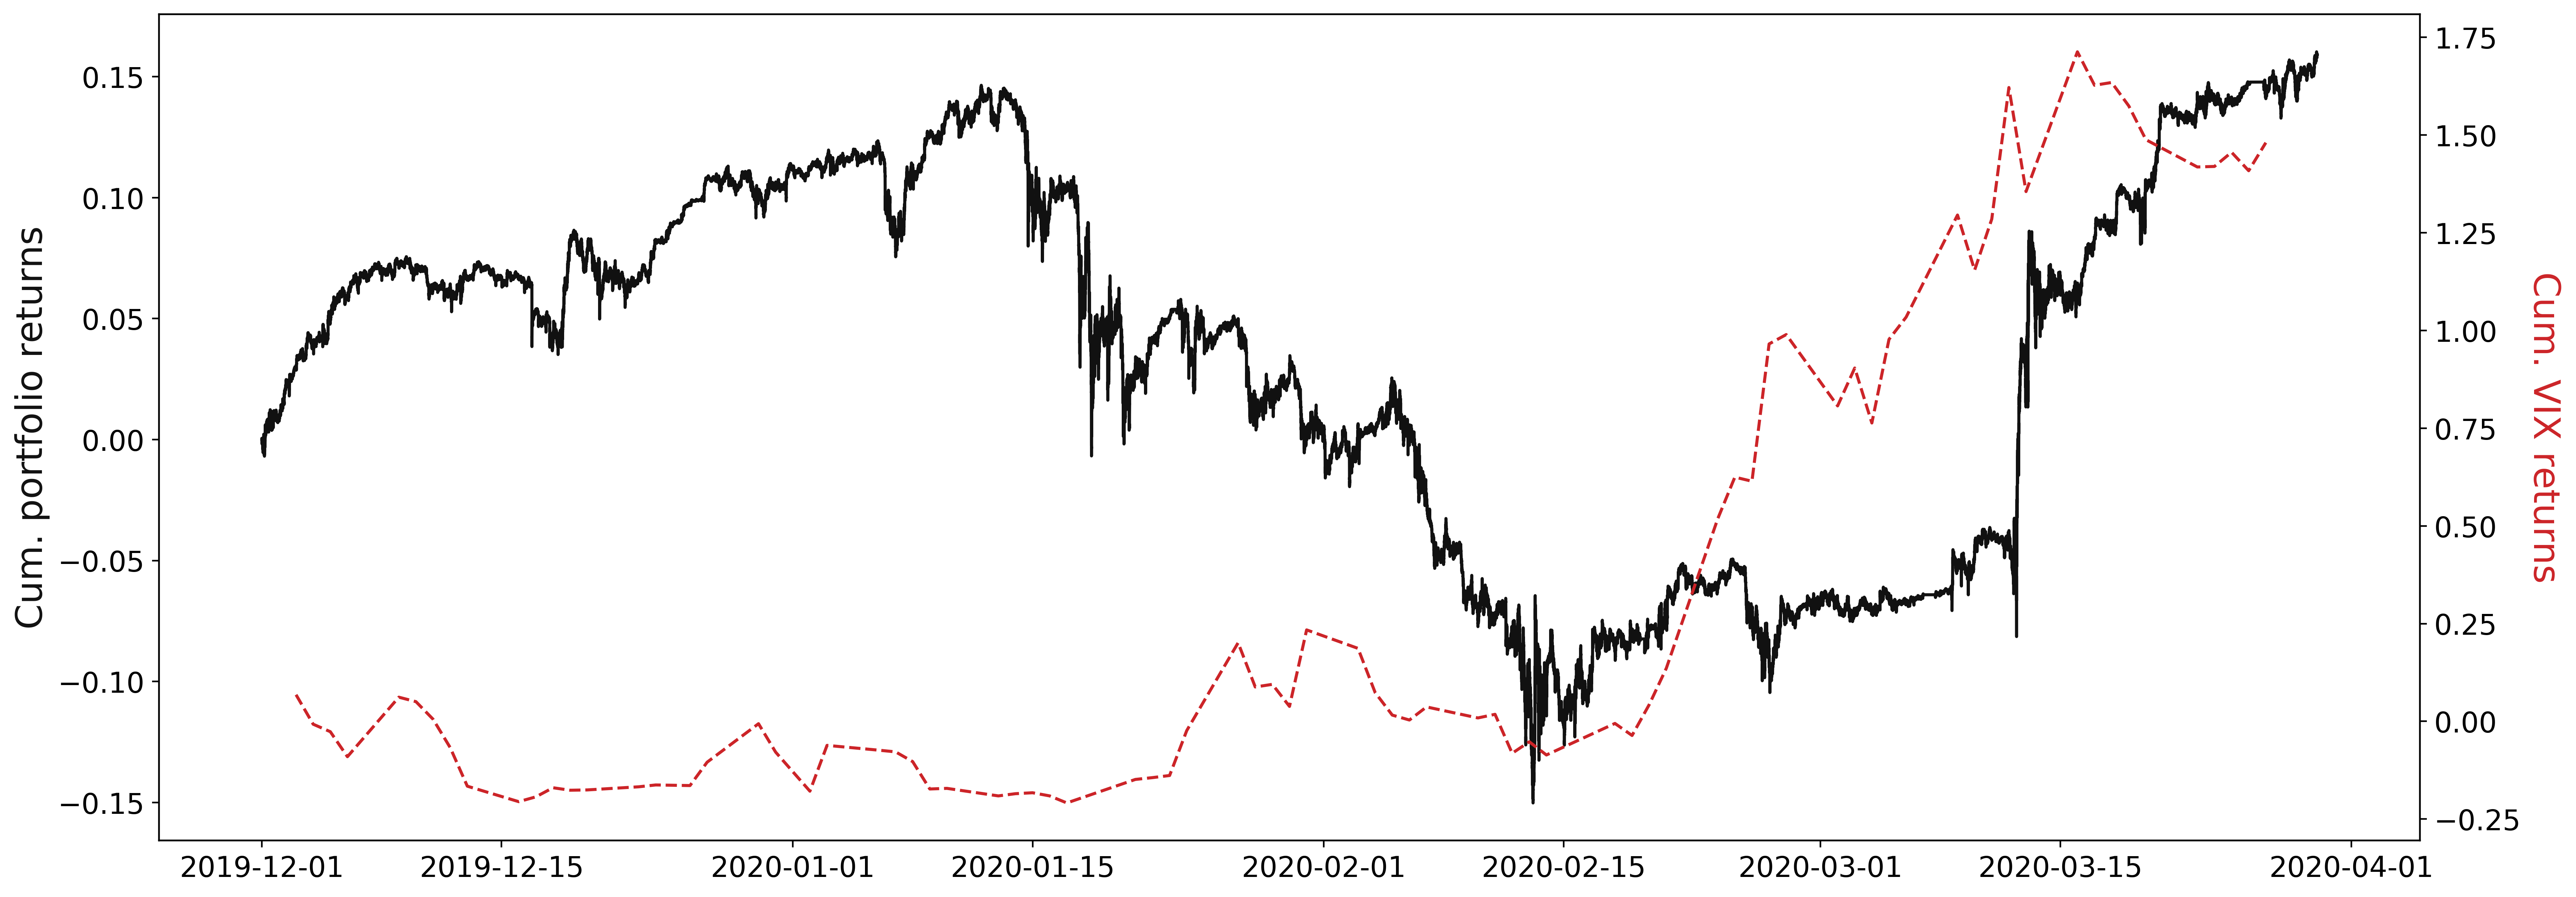
\includegraphics[width=\textwidth,height=\textheight,keepaspectratio]{VIX_vs_PF.png}
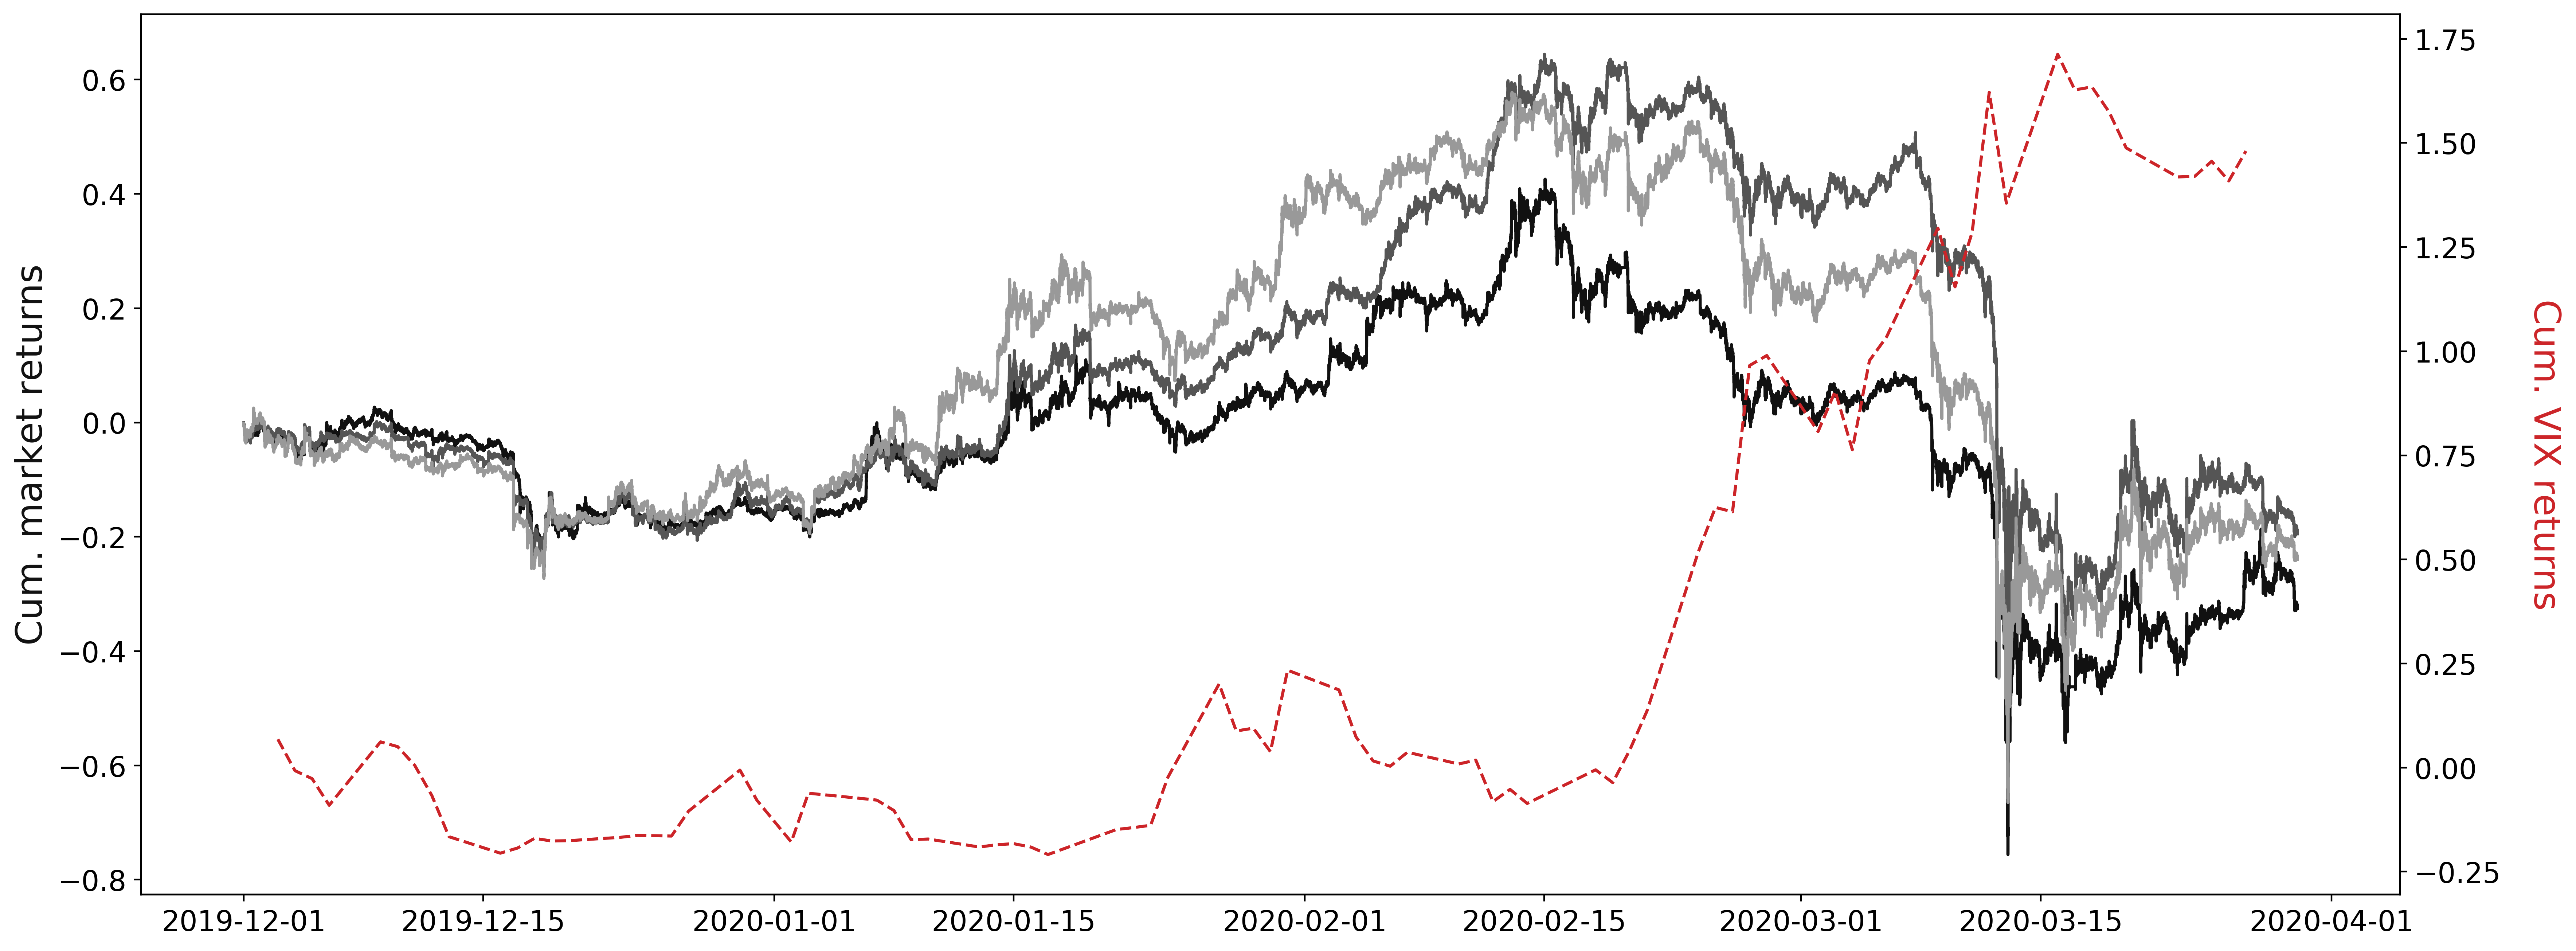
\includegraphics[width=\textwidth,height=\textheight,keepaspectratio]{market_vs_vix.png}
\end{minipage}
\end{center}

The Chicago Board Options Exchange's Volatility index (VIX) is a widely used measure of the market's expectation of volatility, based on implied volatility of S\&P500 options. The index is often used to proxy fear in the market, so when the VIX is high, investors are likely to move away from risky assets such as cryptocurrencies. Akyildirim et al. \citeyear{Akyildirim_2020} find evidence in support of the influence of implied market volatility on cryptocurrency volatility. This is displayed in Figure 9, where it can be observed that the cryptocurrency market is in downturn when the VIX index is high. On the other hand, the portfolio returns seem to be uncorrelated with the VIX returns. In the first month of the backtesting period, the VIX returns remain steady while the trading system is yielding significant profits. When the VIX returns increase over the course of the remaining three months, the trading system is making losses before the returns spike around the middle of March. These findings are in support of diversification benefits that the strategy can provide to equity traders. 

The proposed pair trading system has the ability to generate a positive risk-adjusted return and performs best in a stable market. From the five trading systems that were backtested, the trading system with opening conditions at $\pm$ one standard deviation from the mean yielded the highest risk-adjusted return in terms of the Sharpe ratio and RoMMD. The returns of the strategy show no clear relationship with the returns of the cryptocurrency market or equity market, demonstrating market neutrality to some extent. At the bottom line, the portfolio generated a return of 16.88\% over a period of four months, which is substantially higher compared to the loss-making S\%P500 in the same period.

%###################################################################################################
\section{Extension} \label{sec:Extension}

As an extension to the research, the proposed trading system has been tested with a statistical stop-loss mechanism. The rationale is that the strategy relies on the mean-reversion dynamic of the spread of a cointegrated pair of cryptocurrency exchange rates, and, when this cointegrating relationship dissolves over time, the spread will not mean-revert and hence will lose its ability to lock-in a profit. Open positions in the constituents of a pair that is no longer cointegrated increase opportunity costs and aggravate potential losses. The anticipated benefit of using a statistical stop-loss mechanism over a fixed stop-loss is that it can capture large spread deviations, shown in Figure 4, without issuing an expensive stop-loss order. To the best of my knowledge, this technique has not been explored in the literature to date. 

The proposed solution incorporates daily reevaluation of cointegrating relationships of pairs. In practice, this is done by the means of a daily rolling window of the unit root test, where the spread, $\hat{\epsilon}$ from equation 4, is tested for stationarity by means of the ADF test with 95\% confidence. If the spread is not stationary in the preceding window, the positions in the corresponding pair are closed immediately and the pair is not considered for further trading. If the spread of a pair is stationary in a window thereafter, the pair is considered for trading again. This allows the trading system to cope with changing relationships, which are expected to change over time.

Figure 10 shows the progression of the p-value of the daily conducted ADF tests. A p-value that exceeds the dashed line means that the null hypothesis of the ADF test cannot be rejected given the exchange rate data in the preceding window and implies that the spread of the pair is not stationary anymore. Such failure to reject the null hypothesis occurs when the previously cointegrated exchange rates are drifting apart, e.g. when one of the exchange rates experiences a shock relative to its counterpart. Several cointegrating relationships dissolved around the middle of January and at the same time, a shock occurred in the market as observed in Figure 2. The declining portfolio returns around the same time, observed in Figure 7, are another manifestation of the shock. Around the middle of February, more cointegrating relationships dissolved. A possible explanation is the transition of a bull market to a bear market, as shown in Figure 2 and 7, where the transition occurred at different times for each exchange rate. 

% Figure 10
\begin{center}
\begin{minipage}{\textwidth}
\captionof{figure}{Rolling ADF test}
\caption*{\footnotesize The augmented Dicky-Fuller (ADF) test statistic is estimated in a daily rolling window, looking back one month. The p-value of the test statistic is plotted over time from 01-12-2019 00:00 until 29-03-2020 00:00. Whenever the p-value is beneath the 5\% confidence interval boundary, the null hypothesis is rejected and the spread series doesn't have a unit root, indicating stationarity. If the p-value breaches the 5\% boundary, the null hypothesis is not rejected and the spread series does have a unit root, indicating non-stationarity.}
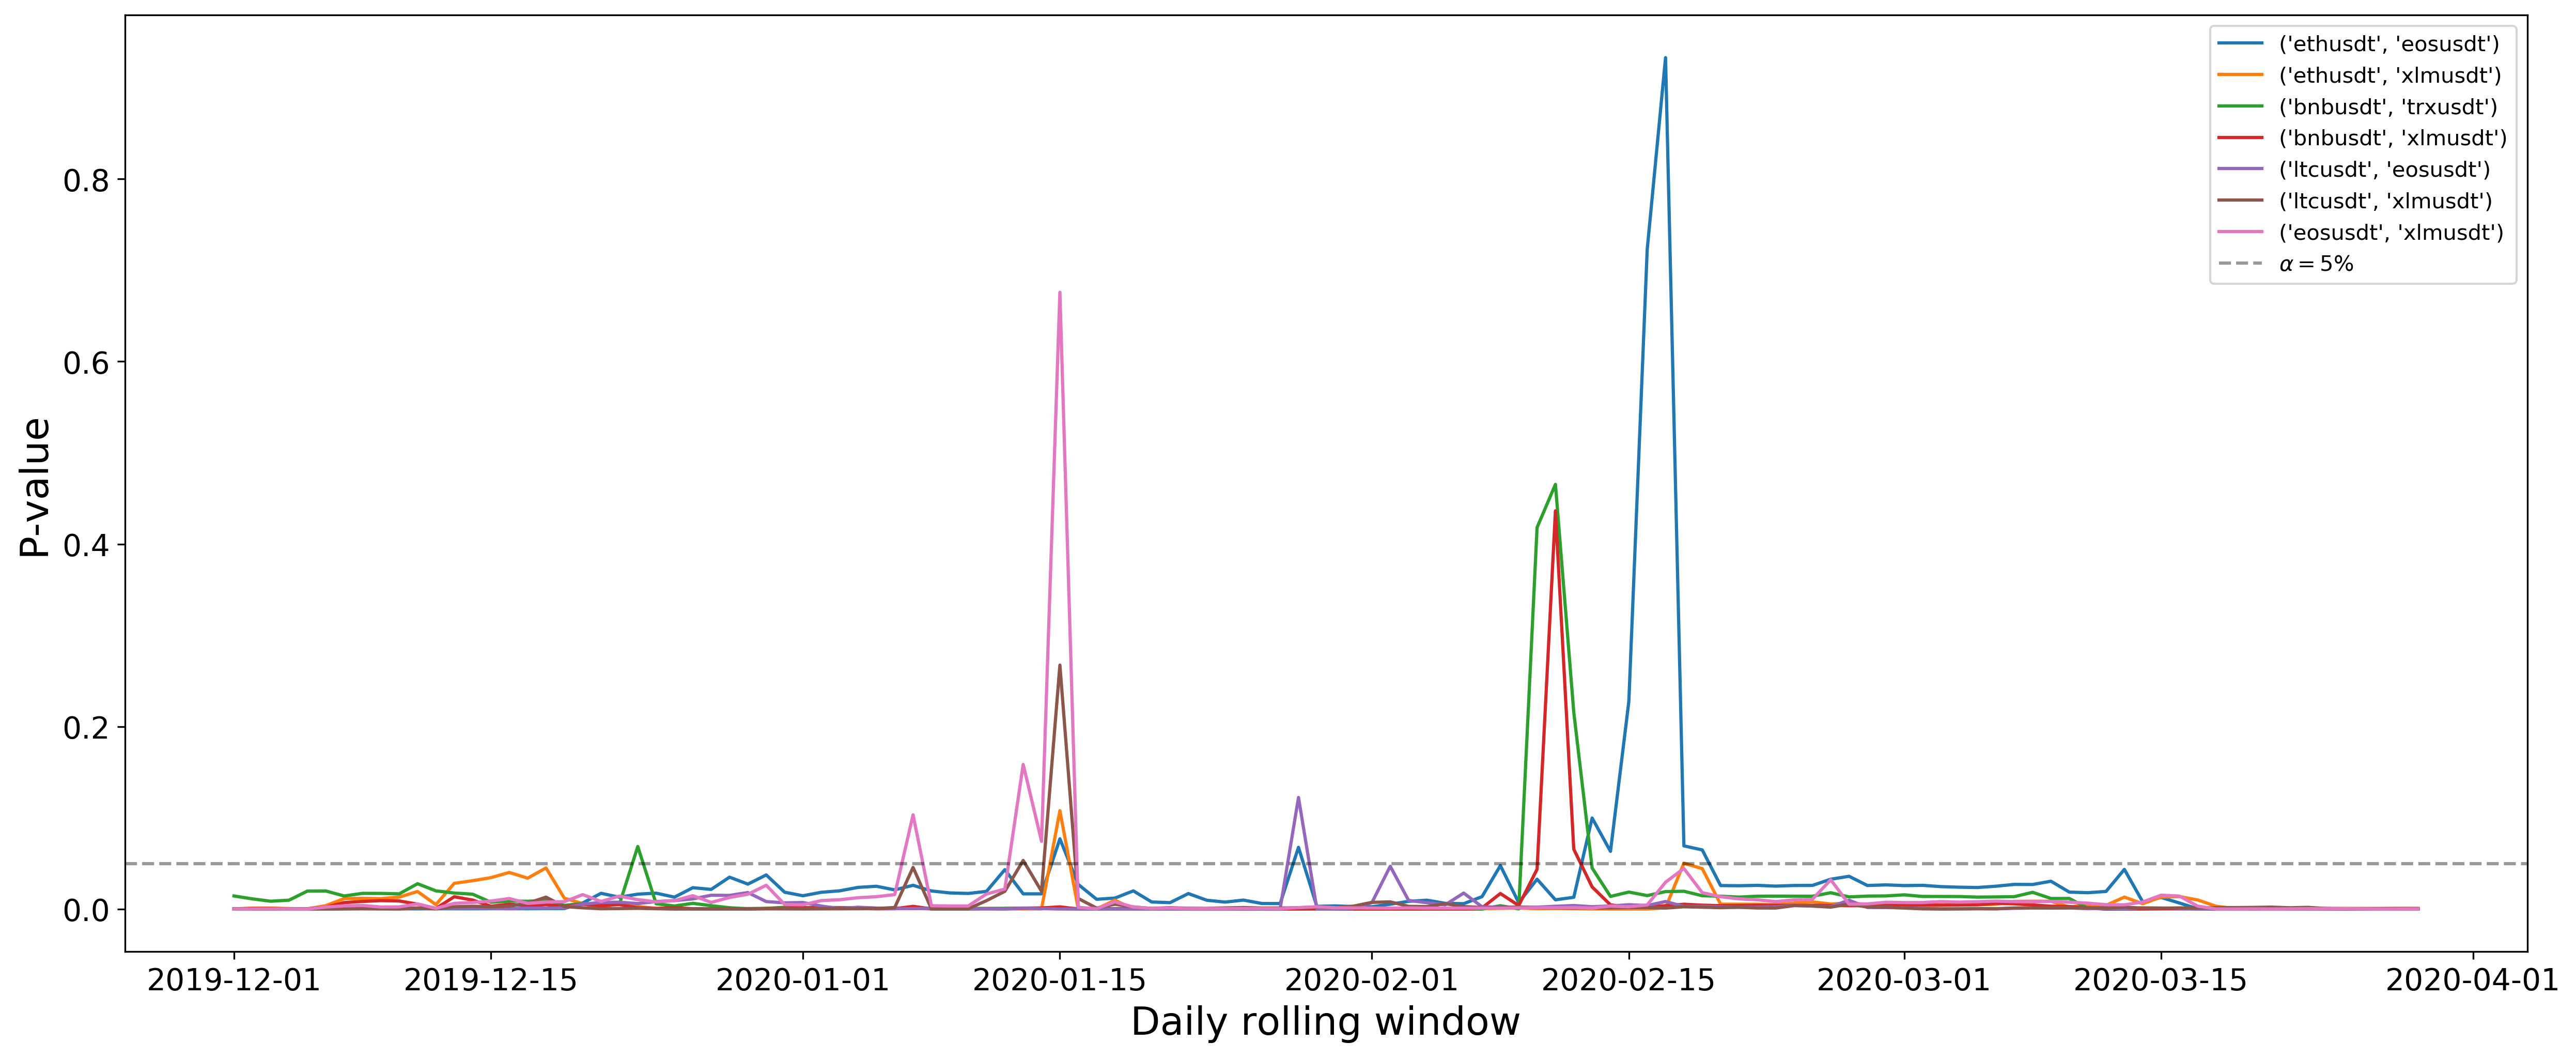
\includegraphics[width=\textwidth,height=\textheight,keepaspectratio]{ADF_pvalues_overtime.png}
\end{minipage}
\end{center}

Table 7 shows the five trading systems with varying thresholds when the statistical stop-loss mechanism is incorporated, without changing anything else. Compared to Table 5, where the results of the trading systems without stop-loss have been summarized, the number of trades significantly increased for trading systems 1 and 3 with roughly 10\% and 20\%, respectively. The portion of winning trades remains almost the same for all five trading systems. Interestingly, the average of losing trades decreased and the maximum drawdown is reduced, indicating that the statistical stop-loss did a good job in limiting losses. Ultimately, the Sharpe ratio is higher for all trading systems except for trading system 3. These findings show the added value of the statistical stop-loss mechanism compared to no stop-loss at all.

% SUMMARY TABLE
\begin{table}[H]
\caption{\label{tab:table-name} Summary of performance}
\caption*{\footnotesize A summary of the performance of the proposed pair trading system in the backtesting period from 01-12-2019 00:00 until 29-03-2020 23:59. Each trade consists of a long and a short position and its profitability is assessed at closing. PnL stands for 'profit-and-loss'. The final return is made up from the cumulative PnL and transaction costs are deducted. The descriptive statistics in the second column have the purpose of describing the weekly PnL measures.}
\begin{tabular*}{\textwidth}{l @{\extracolsep{\fill}} rrrrrr}
\Xhline{2.25\arrayrulewidth}
\thead[l]{Trading system}&\thead{1}&\thead{2}&\thead{3}&\thead{4}&\thead{5}\\
\thead[l]{Threshold}&\thead{\bm{$\pm0.5\sigma$}}&\thead{\bm{$\pm0.75\sigma$}}&\thead{\bm{$\pm \sigma$}}&\thead{\bm{$\pm1.25\sigma$}}&\thead{\bm{$\pm1.5\sigma$}}\\
\Xhline{0.5\arrayrulewidth}
No. Winning trades&481&283&230&179&143\\
No. Losing trades&135&100&91&75&61\\
Total no. Of closed trades&616&383&321&254&204\\
Perc. of winning trades&78.08\%&73.89\%&71.65\%&70.47\%&70.10\%\\
Perc. of losing trades&21.92\%&26.11\%&28.35\%&29.53\%&29.90\%\\
Avg. of winning trades&\$16.48&\$20.67&\$23.29&\$26.96&\$30.09\\
Avg. of losing trades&\$-45.39&\$-49.75&\$-50.55&\$-53.76&\$-58.90\\
Avg. of all trades&\$2.93&\$2.28&\$2.36&\$3.13&\$3.48\\
Mean daily return&0.17\%&0.09\%&0.07\%&0.09\%&0.07\%\\
Median daily return&0.18\%&0.03\%&0.06\%&0.04\%&0.04\%\\
Minimum daily return&-3.86\%&-3.96\%&-479\%&-3.73\%&-3.47\%\\
Maximum daily return&7.94\%&10.38\%&13.69\%&9.37\%&9.17\%\\
Standard deviation&1.59\%&1.63\%&1.92\%&1.46\%&1.43\%\\
MDD&-24.74\%&-23.57\%&-24.24\%&-21.26\%&-18.87\%\\
Annual RoMDD&2.49&1.42&2.08&1.53&1.38\\
Annual Sharpe&2.02&1.07&0.70&1.17&1.17\\
\Xhline{0.5\arrayrulewidth}
Final PnL&\$1790.78&\$933.03&\$841.13&\$905.41&\$713.14\\
\Xhline{1.5\arrayrulewidth}
\end{tabular*}
\end{table}

% % WEEKLY TABLE
% \begin{table}[ht]
% \centering
% \caption{\label{tab:table-name} Weekly performance}
% \caption*{\footnotesize The performance of the proposed high frequency pair trading system in the backtesting period, out-of-sample, from 01-12-2019 00:00 until 29-03-2020 23:59 dissected in weeks. From left to right, the week columns displays the week in which the performance is measured, followed by the total number of trades in that week. Each position consists of a long and short position in the exchange rates that make up a pair. The winning trades column shows the number of positions that have been closed with a profit. The average investment column shows the average outlay of cash per position. The profit-and-loss (PnL) column shows the profits per week in USDT, followed by the best and worst trade in the corresponding week, also denoted in USDT. The bottom row contains column totals and column averages, indicated by * and **, respectively.}
% \resizebox{\textwidth}{!}{\begin{tabular}{lrrrrllll}
% \Xhline{2.25\arrayrulewidth}
% \thead[l]{Week}&\thead{No. of pos.}&\thead{No. of closed pos.}&\thead{No. of successfully closed}&\thead{\% Succesful}&\thead{Avg. cashflow}&\thead{PnL}&\thead{Best}&\thead{Worst}\\
% \Xhline{0.5\arrayrulewidth}
% 48&7&0&0&0\% & \$-232,51& \$0& \$0& \$0\\
% 49&21&11&7&64\% & \$40,02& \$111,16& \$38,48& \$-13,58\\
% 50&25&14&12&86\% & \$-132,17& \$95,44& \$23,28& \$-29,29\\
% 51&42&20&14&70\% & \$-65,15& \$16,02& \$25,02& \$-108,55\\
% 52&38&19&12&63\% & \$64,8& \$213,08& \$160,6& \$-49,1\\
% 1&28&14&12&86\% & \$2,75& \$150,05& \$29,48& \$-20,41\\
% 2&65&32&24&75\% & \$79,74& \$61,91& \$33,96& \$-73,83\\
% 3&84&41&25&61\% & \$155,76& \$-120,1& \$192,61& \$-145,83\\
% 4&43&23&10&43\% & \$-78,54& \$-574,29& \$29,7& \$-282,84\\
% 5&57&28&20&71\% & \$128,25& \$-309,83& \$26,63& \$-120,28\\
% 6&91&45&34&76\% & \$166,23& \$-343,12& \$28,5& \$-147,81\\
% 7&92&47&33&70\% & \$95,85& \$-553,08& \$419,53& \$-694,88\\
% 8&100&50&42&84\% & \$-4,89& \$481,1& \$251,71& \$-115,99\\
% 9&104&52&46&88\% & \$-35,44& \$236,25& \$31,25& \$-101,47\\
% 10&66&32&28&88\% & \$30,24& \$182,93& \$29,24& \$-75,23\\
% 11&142&71&63&89\% & \$-12,5& \$1331,18& \$82,17& \$-187,64\\
% 12&90&46&39&85\% & \$57,42& \$666,63& \$59,79& \$-108,27\\
% 13&37&19&15&79\% & \$45,55& \$222& \$44,03& \$-23,14\\
% \Xhline{0.5\arrayrulewidth}
% \textbf{Avg.*/Sum**}&\textbf{1132**}&\textbf{564**}&\textbf{436**}&\textbf{77\%*} & \textbf{\$16,97*}& & & \\
% \Xhline{1.5\arrayrulewidth}
% \end{tabular}}
% \end{table}

% ############################################################################################################
\section{Conclusion} \label{sec:Conclusion}

Short-term speculation strategies that solely rely on historical data are not expected to yield excess returns in financial markets, because all information is included in prices. The emerging cryptocurrency market, on the other hand, is still in the process of becoming an efficient market \cite{Urquhart_2016, Aggarwal_2019}. This makes it an appealing environment for high frequency traders to seek an edge. In this paper, a high frequency cointegration-based pair trading system is proposed and its ability to generate a positive risk-adjusted return is tested over the course of four months. The paper builds on existing pair trading literature of Vidamurthy \citeyear{Vidamurthy_2004} and Gatev \citeyear{Gatev2006}. Contributions to the literature are made by leveraging minute-binned exchange rate data to profit from short-term deviations of the spread of eight cointegrated pairs of cryptocurrency exchange rates, whereas other studies use daily price data and a smaller set of exchange rates \cite{Leung_2018, Miao_2014}. 

Due to strong signs of comovement and interconnectedness among cryptocurrencies, it was expected to find cointegrated pairs. Despite the strict selection process, eight pairs of exchange rates are determined to be significantly cointegrated. It was also expected that cointegrating relationships change over time, as a consequence of market volatility. In fact, figure 10 shows that the spread is not stationary throughout the complete backtesting period. As an extension, it is found that a statistical stop-loss mechanism, based on a rolling window unit root test, is able to limit losses that arise from changing cointegrating relationships, reducing the maximum drawdown and average of losing trades of the portfolio.

The selected pairs are backtested in five pair trading systems with varying thresholds. The trading system with thresholds at $\pm$ one standard deviation from the mean spread yields the highest risk-adjusted return, proxied by the Sharpe ratio of 1.68 and RoMDD of 2.12. The proposed strategy outperforms the equity market, proxied by the S\&P500 index, which yielded a Sharpe ratio of 0.84 in the past ten years. 

Significant profits were generated during the first month of the backtesting period, when the market was stable. The trading system made losses during the two subsequent months when the market was unstable, followed by one month in which the losses were mitigated by a series of profitable trades when the exchange rates stabilised. Moreover, the portfolio returns are not correlated to the equity market and the cryptocurrency market, hence the high frequency pair trading system demonstrates market neutrality to some extent and provides diversification opportunities to investors. 

% limitations
The research has potential limitations that need to be addressed. The data set used in this research is relatively short, so it remains unknown if the trading system accomplishes the same results in a different market scenario. This is partially mitigated by the fact that the data set incorporates a calm and stressed period. The infancy of the cryptocurrency market poses a challenge that can only be overcome by time, as the universe of cryptocurrencies expanded substantially in 2018, the data that is available for many of the exchange rates that are considered in this paper is limited. On the other hand, it is possible that a new blockchain foundation will be created in the near future, giving rise to a number of new cryptocurrencies accompanied by new trading opportunities. A similar event occurred in 2017, when the market was flooded with altcoins that are based on the Ethereum blockchain.

To make the research fully consistent, the pair trading system should identify cointegrated pairs among the complete set of cryptocurrency exchange rates in a rolling window. Due to limited computing power, this was not possible, and the pair trading system only included the eight pairs that were identified in the first month of the data set. It is expected that the ability of the high frequency pair trading system to generate risk-adjusted returns would be aggravated without this limitation, primarily because it would be able to grasp more trading opportunities. This leaves opportunities for further research. 

Moreover, the results are based on the assumption that limit orders get filled instantaneously. Even though the cryptocurrencies chosen for trading are the most liquid ones among all the cryptocurrencies offered on the Binance exchange, it can occur that a limit order does not get filled and, as a consequence, the results would be different compared to the results presented in this paper. A way to assure that orders are filled is using market orders, but this would come with additional trading costs that arise from crossing the spread. 
% limitations
 
From the findings, it can be concluded that a high frequency cointegration-based pair trading system has the ability to yield a risk-adjusted return in the cryptocurrency market. This puts doubt on weak-form market efficiency of the cryptocurrency market, which is consistent with earlier research. The findings of this paper may be valuable to (high frequency) traders who seek an edge in the emerging cryptocurrency market through the implementation of a pair trading strategy.

\bibliographystyle{apacite}
\bibliography{references}

\end{document}
